% \documentclass[ba,preprint]{imsart}% use this for supplement article
\documentclass[aoas,preprint]{imsart}

%% Packages
\RequirePackage{amsthm,amsmath,amsfonts,amssymb,mathtools}
%\RequirePackage[numbers]{natbib}
\RequirePackage[authoryear]{natbib}%% uncomment this for author-year citations
\RequirePackage[colorlinks,citecolor=blue,urlcolor=blue,filecolor=black,backref=page]{hyperref}
\usepackage[ruled,vlined,linesnumbered]{algorithm2e}
\usepackage{bbm}
\newcommand\given[1][]{\:#1\vert\:}
\newcommand{\dd}{\mathop{}\!\mathrm{d}}
\RequirePackage{graphicx}
\usepackage{multirow}
\usepackage{float}
\usepackage{forest}
\usepackage{threeparttable}
\usepackage{caption}
\usepackage{subcaption}
\usepackage{etoolbox}
\usepackage{anyfontsize}
\usepackage{comment}
\usepackage{enumitem}
\AtBeginEnvironment{algorithm}{\linespread{0.8}\selectfont}
\pubyear{2024}
%\arxiv{2024.00000}
\volume{TBA}
\issue{TBA}
\firstpage{1}
\lastpage{1}


\startlocaldefs
%%%%%%%%%%%%%%%%%%%%%%%%%%%%%%%%%%%%%%%%%%%%%%
%%                                          %%
%% Uncomment next line to change            %%
%% the type of equation numbering           %%
%%                                          %%
%%%%%%%%%%%%%%%%%%%%%%%%%%%%%%%%%%%%%%%%%%%%%%
%\numberwithin{equation}{section}
%%%%%%%%%%%%%%%%%%%%%%%%%%%%%%%%%%%%%%%%%%%%%%
%%                                          %%
%% For Axiom, Claim, Corollary, Hypothesis, %%
%% Lemma, Theorem, Proposition              %%
%% use \theoremstyle{plain}                 %%
%%                                          %%
%%%%%%%%%%%%%%%%%%%%%%%%%%%%%%%%%%%%%%%%%%%%%%
\newcommand*\samethanks[1][\value{footnote}]{\footnotemark[#1]}
\theoremstyle{plain}
\newtheorem{axiom}{Axiom}
\newtheorem{claim}[axiom]{Claim}
\newtheorem{theorem}{Theorem}[section]
\newtheorem{lemma}[theorem]{Lemma}
%%%%%%%%%%%%%%%%%%%%%%%%%%%%%%%%%%%%%%%%%%%%%%
%%                                          %%
%% For Assumption, Definition, Example,     %%
%% Notation, Property, Remark, Fact         %%
%% use \theoremstyle{definition}            %%
%%                                          %%
%%%%%%%%%%%%%%%%%%%%%%%%%%%%%%%%%%%%%%%%%%%%%%
\theoremstyle{definition}
\newtheorem{definition}[theorem]{Definition}
\newtheorem*{example}{Example}
\newtheorem*{fact}{Fact}
%%%%%%%%%%%%%%%%%%%%%%%%%%%%%%%%%%%%%%%%%%%%%%
%%                                          %%
%% For Case use \theoremstyle{remark}       %%
%%                                          %%
%%%%%%%%%%%%%%%%%%%%%%%%%%%%%%%%%%%%%%%%%%%%%%
\theoremstyle{remark}
\newtheorem{case}{Case}
%%%%%%%%%%%%%%%%%%%%%%%%%%%%%%%%%%%%%%%%%%%%%%
%% Please put your definitions here:        %%
%%%%%%%%%%%%%%%%%%%%%%%%%%%%%%%%%%%%%%%%%%%%%%
\endlocaldefs

\begin{document}

\begin{frontmatter}
\title{Seemingly unrelated Bayesian additive regression trees for cost-effectiveness analyses in healthcare}
%\title{A sample article title with some additional note\thanksref{t1}}
\runtitle{Seemingly unrelated BART}
%\thankstext{T1}{A sample additional note to the title.}

\begin{aug}
%%%%%%%%%%%%%%%%%%%%%%%%%%%%%%%%%%%%%%%%%%%%%%%
%% Only one address is permitted per author. %%
%% Only division, organization and e-mail is %%
%% included in the address.                  %%
%% Additional information can be included in %%
%% the Acknowledgments section if necessary. %%
%% ORCID can be inserted by command:         %%
%% \orcid{0000-0000-0000-0000}               %%
%%%%%%%%%%%%%%%%%%%%%%%%%%%%%%%%%%%%%%%%%%%%%%%
\author[A]{\fnms{\textbf{Jonas}}~\snm{\textbf{Esser}}{\footnotesize\textsuperscript{\!,\!}}\ead[label=e1]{j.esser@vu.nl}\orcid{0009-0005-4964-5525}},
\author[B]{\fnms{\textbf{Mateus}}~\snm{\textbf{Maia}}\samethanks{\footnotesize\textsuperscript{\!,\!}}\ead[label=e2]{mateus.maiamarques@glasgow.ac.uk}\orcid{0000-0001-7056-386X}},
\author[C]{\fnms{Andrew C.}~\snm{Parnell}\ead[label=e3]{andrew.parnell1@ucd.ie}\orcid{0000-0001-7956-7939}},
\author[A]{\fnms{\linebreak{}Judith E.}~\snm{Bosmans}\ead[label=e4]{j.e.bosmans@vu.nl}\orcid{0000-0002-1443-1026}},
\author[A]{\fnms{Johanna Maria}~\snm{van Dongen}\ead[label=e5]{j.m.van.dongen@vu.nl}\orcid{0000-0002-1606-8742}},
\author[D]{\fnms{Thomas}~\snm{Klausch}\ead[label=e6]{t.klausch@amsterdamumc.nl}},
\and
\author[E]{\fnms{Keefe}~\snm{Murphy}\ead[label=e7]{keefe.murphy@mu.ie}\orcid{0000-0002-7709-3159}}
%%%%%%%%%%%%%%%%%%%%%%%%%%%%%%%%%%%%%%%%%%%%%%
%% Addresses                                %%
%%%%%%%%%%%%%%%%%%%%%%%%%%%%%%%%%%%%%%%%%%%%%%

\address[A]{Faculty of Science, Health Economics and Health Technology Assessment, Vrije Universiteit Amsterdam,\linebreak{}\printead[presep={}]{e1,e4,e5}}

\address[B]{School of Mathematics and Statistics, University of Glasgow,\printead[presep={}]{e2}}

\address[C]{School of Mathematics and Statistics, Insight Centre for Data Analytics, University College Dublin,\printead[presep={}]{e3}}

\address[D]{Department of Epidemiology and Data Science, Amsterdam University Medical Center,\printead[presep={}]{e6}}

\address[E]{Hamilton Institute and Department of Mathematics and Statistics, Maynooth University,\printead[presep={}]{e7}}

\runauthor{Esser, Maia, et al.}

\end{aug}

\begin{abstract}
In recent years, theoretical results and simulation evidence have shown Bayesian additive regression trees to be a highly-effective method for nonparametric regression. Motivated by cost-effectiveness analyses in health economics, where interest lies in jointly modelling the costs of healthcare treatments and the associated health-related quality of life experienced by a patient, we propose a multivariate extension of BART which is applicable in regression analyses with several dependent outcome variables.
Our framework allows for continuous or binary outcomes and overcomes some key limitations of existing multivariate BART models by allowing each individual response to be associated with different ensembles of trees, while still handling dependencies between the outcomes. In the case of continuous outcomes, our model is essentially a nonparametric version of seemingly unrelated regression. Likewise, our proposal for binary outcomes is a nonparametric generalisation of the multivariate probit model. We give suggestions for easily interpretable prior distributions, which allow specification of both informative and uninformative priors.
We provide detailed discussions of MCMC sampling methods to conduct posterior inference. Our methods are implemented in the \textsf{R} package \texttt{subart}. We showcase their performance through extensive simulation experiments and an application to an empirical case study from health economics. By also accommodating propensity scores in a manner befitting a causal analysis, we find substantial evidence for a novel trauma care intervention's cost-effectiveness.
\end{abstract}

\begin{keyword}
\kwd{Bayesian additive regression trees}
\kwd{causal inference}
\kwd{cost-effectiveness}
\kwd{health economics}
\kwd{multivariate probit}
\kwd{seemingly unrelated regression}
\end{keyword}

\end{frontmatter}

\section{Introduction}
Many research questions in health economics are concerned with trading off the costs and benefits of a medical intervention. The most prominent examples are in \textit{cost-effectiveness analysis} (CEA), where we wish to decide whether a new innovative treatment is worth the associated increase in costs compared to usual care. We thus need to estimate the average treatment effects on both costs and health. However, in order to get coherent measures of uncertainty, the two treatment effects must be estimated jointly in order to account for the correlation between them \citep{baio2012bayesian}. Furthermore, if the CEA is performed with observational data, where the treatment assignment is not randomised, we additionally have to adjust for confounding bias in the analysis. These points are elaborated in Section \ref{sec:application}.

In this paper we aim to estimate the cost-effectiveness of a novel treatment for physical trauma rehabilitation, called the \textit{transmural trauma care model} (TTCM), using data gathered under a study by \citet{wiertsema2019cost} which we will henceforth refer to as the \textit{TTCM data}. The treatment assignment is not randomised and the number of potential confounders is large relative to the sample size. Of the multiple cost and effectiveness outcomes the authors investigated, we focus on healthcare-related costs and health-related quality of life. It is of interest to jointly estimate both outcomes, and reasonable to assume both that the outcomes are non-linearly related to the available predictors and that each outcome may depend on different subsets of predictors, which may in turn interact in complex ways. The challenge of CEA under these circumstances motivated the development of our novel methodology, though we also anticipate its use in other CEA studies and broader healthcare settings.

%In the causal inference literature, 
There is wide agreement in the causal inference literature that flexible nonparametric methods, which do not impose strong %parametric 
assumptions on the regression functions, are the best tools for estimating treatment effects with observational data \citep{dorie2019automated,rudolph2023all}. It is not straightforward, however, to apply this knowledge in the context of CEAs. Seemingly unrelated regression  models \citep[SUR;][]{zellner1962efficient}, the most recommended statistical method for CEAs \citep{willan2004regression,el2022scoping}, impose strong linearity assumptions, which can bias the inferences if there are strong non-linear relationships between the variables of interest. On the other hand, there is a distinct lack of nonparametric regression methods which can handle multivariate outcomes. We adopt a Bayesian perspective and fill this gap by developing a nonparametric version of SUR, which replaces the linear predictors in the SUR model by sums of regression trees. In the univariate case, this regression method has become known as \textit{Bayesian additive regression trees} (BART). BART has already demonstrated competitive performance for univariate responses \citep{dorie2019automated,rudolph2023all} and it seems plausible that this efficacy will extend to situations with multiple outcomes of interest. However, by embedding BART in the SUR framework, we also seek to overcome some limitations of existing multivariate BART extensions.

\citet{chipman2010bart} introduced BART as an ensemble method, where each learner is a tree following the Bayesian CART approach previously proposed by the same authors \citep{chipman1998bayesian}. Considering a univariate response vector $\mathbf{y} \in \mathbb{R}^{n}$ and a set of predictors $\mathbf{X} \in \mathbb{R}^{n\times p}$, which may be of mixed type, the main objective of regression modelling is to estimate the conditional expectation $\mathbb{E}\lbrack y_i\given \mathbf{x}_i\rbrack$. As a nonparametric model, BART offers high flexibility in estimating this regression function. The tendency of decision trees to overfit is mitigated by the Bayesian underpinnings of the method, allowing informative prior distributions to impose regularisation in a principled and transparent fashion, as well as the additive nature of the ensemble. These features facilitate better generalisation, in a similar vein to the gradient boosting approach of \citet{friedman2001greedy}. The success of BART is widely reported in the literature across a broad spectrum of applications \citep{janizadeh2021novel,sarti2023bayesian,yee2024evaluating}. In addition, theoretical work has demonstrated the frequentist optimality of BART under certain conditions \citep{linero2018bayesian,rockova2020semi,rockova2020posterior}.

The BART model was originally developed for univariate responses but subsequent extensions emerged to adapt BART to multivariate responses, such as the Bayesian additive vector autoregressive tree \citep{florian2022vabart} for multivariate time-series and formulations by \citet{peruzzi2022spatial} for multivariate spatial data. Other applied work involves an extension of BART to forecast the tails of multivariate responses \citep{clark2023tail}. \citet{um2023bayesian} adapted BART to cover not only multivariate responses but also the assumption of a skew-normal distribution; throughout this paper, we refer to the non-skewed variant as mvBART. Furthermore, \citet{mcjames2024bayesian} proposed an extension of Bayesian causal forests \citep[BCF;][]{hahn2020bayesian} for multivariate responses. All  aforementioned approaches share the limitation that the tree structure must be identical for each component of the outcome vector. It is easy to envisage situations for which this is inappropriate, whereby a specific covariate may be strongly associated with one outcome but independent of another. For example, factors which govern costs may be unrelated to quality of life, and \textit{vice versa}.

In this study we propose a novel variant of BART termed seemingly unrelated BART (suBART) which is designed to handle multivariate continuous responses and address this key limitation. \citet{chipman2010bart} previously drew parallels to SUR models \citep{zellner1962efficient} and alluded to the potential for extending BART in this direction. Our framework differs from the aforementioned multivariate BART extensions, which assume a single set of trees with correlated multivariate leaf node parameters. Instead, we jointly fit an individual ensemble of trees for each outcome and model their interdependence through correlated error terms. Thus, suBART also differs from merely applying univariate BART models to each outcome independently. Motivated by our investigation into the cost-effectiveness of the TTCM intervention, we further extend suBART to incorporate propensity scores, in the spirit of \citet{hahn2020bayesian}, as befits causal analyses. Beyond CEA settings, we also develop probit suBART, an extension of suBART to accommodate multivariate binary outcomes. While not the main focus of this paper, we envision this version of the model being useful in marketing applications with correlated binary outcomes; see the examples in \citet{rossi2005bayesian}. Our approach is similar to that of \citet{chakraborty2016bayesian}, who offers a version of seemingly unrelated BART for exclusively continuous outcomes with an adaptive number of trees. However, it is not specifically tailored to causal inference objectives typical of CEA and lacks an available open-source software implementation. Moreover, the non-informative inverse-Wishart prior adopted by \citet{chakraborty2016bayesian} on the covariance matrix of the error terms fails to properly calibrate the prior on the residual variance parameters, which is crucial for regularising the contributions of the trees in the ensemble. We address these gaps by providing a comprehensive framework, which covers either continuous or binary outcomes, with appropriately specified priors, and a practical implementation through an \textsf{R} package named \texttt{subart}, which is implemented using \texttt{Rcpp} and available at: \url{https://github.com/MateusMaiaDS/subart}.

This article proceeds as follows: Section \ref{sec:application} provides background theory on CEA and motivates the development of suBART in the context of the application to the TTCM data from \citet{wiertsema2019cost}. Section \ref{sec:suBART}  elaborates on the theoretical underpinnings of suBART and Section \ref{sec:posterior} discusses the posterior inference for both the continuous and  binary multivariate outcome settings. Section \ref{sec:simstudies} considers different simulation scenarios to compare the predictive performance of suBART against standard competitors. Section \ref{sec:case_study} presents the empirical findings of our application of suBART to the TTCM data, along with an additional simulation experiment based on these data which assesses suBART's estimation of treatment effects in the CEA setting. Finally, Section \ref{sec:conclusion} summarises the proposed methodologies, highlighting both 
limitations and potential for further extension, and presents conclusions regarding the CEA application. Additional results, comparisons, and findings are included in the Appendices, all of which have been deferred to the Supplementary Material \citep{EsserMaiaSupplement}.

\section{CEA and the suBART model}\label{sec:application}

Our main motivation in developing suBART is its potential applicability in cost-effectiveness analyses of healthcare treatments, particularly in cases where the treatment assignment is not randomised. When estimating treatment effects from such observational data, simple parametric models often lead to severe bias and flexible nonparametric models are preferable \citep{hernan2024causal}. 
Naturally, such concerns extend to CEA settings, where we want to estimate two treatment effects simultaneously. However, there is a lack of statistical methods fit for such purposes. Given that BART has proven to be very useful for univariate causal inference tasks \citep{hill2011bayesian,dorie2019automated,rudolph2023all}, we consider it a promising basis for multivariate CEA.

We continue by sketching some relevant ideas from health economics and causal inference in Section \ref{sec:CEA_theory}, drawing on the detailed treatments found in \citet{gabrio2019bayesian} and \citet{li2023bayesian}. Subsequently, we give a detailed presentation of the TTCM data in Section \ref{sec:TTCM_intro}.

\subsection{Cost-effectiveness analyses with observational data}\label{sec:CEA_theory}

The fundamental problem of CEA in health economics is to determine which of two competing healthcare treatments (usually, but not always, for the same disease) should be implemented. Often one is both more effective and more expensive than the other, which raises the question whether the increase in health is worth the added expenses. Henceforth, we let $c_i$ and $q_i$ denote the healthcare costs and health-related quality of life of a given patient, respectively, and let $t = 0$ and $t = 1$ denote the two different treatments of interest. Using the usual potential outcomes notation, we let $c_i(t)$ denote the costs associated with patient $i$, had they received treatment $t$ and do likewise for $q_i(t)$. We further suppose that there is some vector of baseline characteristics $\mathbf{x}_i$ which have an effect on both the outcomes $c_i$ and $q_i$, as well as the treatment indicator $t_i$.

Given a sample of $n$ observations, we wish to estimate the \textit{mixed average treatment effect} (MATE)\footnote{The naming of treatment effects is inconsistent in the literature. This has been referred to as the \textit{population average treatment effect} (PATE) by \citet{imbens2015pate} and others. We adopt the MATE terminology in the sense of \citet{li2023bayesian}, whose definition of the PATE requires a generative model for the covariates.}
on the costs in this sample, which we define as 
\begin{equation}\Delta_c \coloneqq \frac{1}{n} \sum^n_{i = 1} \mathbb{E}\left\lbrack c_i(1)\given \mathbf{x}_i\right\rbrack -  \mathbb{E}\left\lbrack c_i(0)\given \mathbf{x}_i\right\rbrack.\label{eq:li_MATE}
\end{equation}
We now make the assumption of \textit{ignorability}, which means that conditional on the baseline covariates $\mathbf{x}_i$, the treatment $t_i$ is independent of the potential outcomes $c_i(0)$ and $c_i(1)$. Under this assumption, we may rewrite our treatment effect as 
\[\Delta_c = \frac{1}{n} \sum^n_{i = 1} \mathbb{E}\left\lbrack c_i\given t_i = 1, \mathbf{x}_i\right\rbrack -  \mathbb{E}\left\lbrack c_i\given t_i = 0, \mathbf{x}_i\right\rbrack.\]
Thus, $\Delta_c$ is completely specified by the conditional expectations $\mathbb{E}\lbrack c_i\given t_i, \mathbf{x}_i\rbrack$. 
We proceed in the same manner for $\Delta_q$, the MATE on the patient's quality of life. It is then customary to combine the two treatment effects into a utility function, the incremental net benefit (INB) as
$\operatorname{INB}_{\lambda} \coloneqq \lambda \Delta_q - \Delta_c.$
The scalar parameter $\lambda$ is called the \textit{willingness-to-pay}. Roughly speaking, $\lambda$ quantifies how much cost (in the given currency) a decision-maker is willing to trade for a one-unit increase in healthcare-related quality of life for one patient. The decision rule is then simple: if the INB is at most zero, we say that treatment $1$ is not cost-effective, and treatment $0$ should be implemented. If the INB is larger than zero, we consider treatment $1$ to be cost-effective and worthy of being implemented. Throughout this paper, we give $\lambda$ values in units of €1,000.

To illustrate the importance of modelling the two outcomes $c$ and $q$ jointly, let us assume for simplicity that the joint distribution of $\Delta_c$ and $\Delta_q$ is bivariate normal. We hence have that
\[
\Pr\left(\operatorname{INB}_{\lambda} > 0\right) = \Phi\!\left(\!\frac{\mathbb{E}\!\left\lbrack \operatorname{INB}_{\lambda} \right\rbrack}{\sqrt{\operatorname{Var}\!\left\lbrack \operatorname{INB}_{\lambda} \right\rbrack}}\!\right) = \Phi\!\left(\!\frac{\lambda \mathbb{E}\!\left\lbrack \Delta_q \right\rbrack - \mathbb{E}\!\left\lbrack \Delta_c \right\rbrack}{\sqrt{\left(\lambda^2 \operatorname{Var}\!\left\lbrack \Delta_q \right\rbrack + \operatorname{Var}\!\left\lbrack \Delta_c \right\rbrack - 2 \lambda \operatorname{Cov}\!\left\lbrack \Delta_q, \Delta_c \right\rbrack \right)}}\!\right).
\]
Consequently, the probability of cost-effectiveness depends on the covariance of $\Delta_c$ and $\Delta_q$. Without the normality assumption, this probability can usually not be found explicitly, but the same principle applies nonetheless: the probability of cost-effectiveness depends on the joint distribution of $\Delta_c$ and $\Delta_q$ \citep{lothgren2000definition, gabrio2019bayesian}. It follows that we must model $c_i$ and $q_i$ jointly, as modelling them separately would enforce the unrealistic assumption that the treatment effects $\Delta_c$ and $\Delta_q$ are independent. This belief is seldom appropriate, since empirical cost and health data are often strongly correlated \citep{willan2004regression}. We expound on these points through simulation experiments in Appendix~A.

We hence use the suBART model developed below to jointly estimate the conditional expectations $\mathbb{E}\lbrack c_i\given t_i, \mathbf{x}_i\rbrack$ and $\mathbb{E}\lbrack q_i\given t_i, \mathbf{x}_i\rbrack$. The treatment effects and INB can then be obtained as functions of these estimates. Our approach mirrors that of \citet{hahn2020bayesian}: we first estimate propensity scores (using probit BART), and then condition the suBART model on all covariates, the treatment indicator, and the estimated propensity scores.

\subsection{Transmural Trauma Care Model (TTCM)}\label{sec:TTCM_intro}

Our data, pertaining to $n=140$ patients suffering from traumatic injuries, were originally collected and analysed by \citet{wiertsema2019cost}. The treatment options, whose assignment was not randomised, are usual care and the novel Transmural Trauma Care Model (TTCM), denoted by $t=0$ and $t=1$, respectively. 
We use the costs from the healthcare perspective ($c_i$) and generic healthcare-related quality of life ($q_i$) as our outcomes. As is usual in CEAs, the former is an aggregate measure: $c_i$ comprises the actual cost of the TTCM intervention (which averages €272 per patient, for those who received it) as well as costs acquired from hospital records. Additionally, several questionnaires were conducted over the course of nine months following treatment, in which patients were surveyed on their use of various healthcare resources. The responses, which relate to issues such as hospital stays, medication use, and surgeries, were then converted to costs and also included in $c_i$. Conversely, $q_i$ was calculated from one single survey administered nine months after treatment using the EQ-5D-3L instrument \citep{lamers2006dutch}.

The data also include $p=11$ baseline covariates, with respective sample sizes of $83$ and $57$ in the two treatment groups. The ratio of covariates to observations is thus reasonably large. We have the following continuous covariates: \textit{age}, \textit{injury severity score}, \textit{length of hospital stay} (in days), and \textit{TTO} (days between trauma and first outpatient consultation). Categorical covariates are also available: \textit{gender} (male/female) and \textit{hospital admission} are binary;  while \textit{education level} is ordinal and \textit{fracture region}, \textit{medical history}, and \textit{trauma type} are unordered.

The original dataset had some missing observations (for survey items related to the outcome variables only) which \citet{wiertsema2019cost} dealt with through multiple imputation. Although hospital records were available for all patients, $17\%$ of patients did not complete any follow-up questionnaires and hence were missing all information on $q_i$ and some survey information on $c_i$. Additionally, $39\%$ and $7\%$ of respondents were missing some (but not all) survey items related to $c$ and $q$, respectively. As missing data is not the subject of this paper, we avoid this complication by simply using \textit{one} imputed dataset, obtained through predictive mean matching \citep{vink2014predictive}, and treating that as complete data. Specifically, the imputation is applied to the missing survey items prior to the calculation of $c$ and $q$. The imputation was done using the \texttt{mice} package in \textsf{R} \citep{van2011mice}, with default settings for everything other than setting the imputation method to predictive mean matching.
It follows that our analyses of these data are not directly comparable to the original one in \citep{wiertsema2019cost} and we do not claim that ours are more valid in this regard. We discuss this issue further in Section \ref{sec:conclusion}.

The statistical analysis in \citet{wiertsema2019cost} is based on simple linear models --- more specifically: the SUR model, as presented in Section \ref{sec:suBART_continuous} --- without any interaction terms or other transformations of the covariates. This imposes rather strong assumptions on the regression functions, which we find difficult to justify and, as alluded to in the Introduction, violations of these assumptions can lead to severely biased results. We hence found it necessary to develop the more flexible suBART model, which allows us to jointly estimate both treatment effects without strong functional assumptions.

\section{The suBART models for continuous and binary responses}\label{sec:suBART}
We start by reviewing the original BART model in the univariate setting in Section \ref{sec:review_BART}, in order to provide context for what is to follow. We then present our novel extensions to the multivariate continuous outcome setting in Section \ref{sec:suBART_continuous} and the multivariate binary outcome setting in Section \ref{sec:suBART_probit}. Specific details regarding posterior inference for suBART models are deferred to Section \ref{sec:posterior}.

\subsection{A review of univariate BART}\label{sec:review_BART} 
BART was designed to solve the classic regression problem of the form
$y_i = \mathbb{E}\left\lbrack y_i\given \mathbf{x}_i\right\rbrack + \varepsilon_i$,
where $y_i$ is a univariate response variable for observation $i=1,\ldots,n$, $\mathbf{x}_i$ is a $p$-dimensional predictor, and $\varepsilon_i \sim \operatorname{N}(0,\sigma^2)$. The idea is to find a flexible approximation for the conditional expectation $\mathbb{E}\lbrack y_i\given \mathbf{x}_i\rbrack$ by expressing it as a sum of regression trees.
A regression tree consists of two components:
\begin{enumerate}
    \item A binary tree $\mathcal{T}$, which defines a finite partition $\{\mathcal{A}_1,\ldots,\mathcal{A}_h\}$ of $\mathbb{R}^p$ based on the feature space of $\mathbf{X}$, using the available predictors 
    to form splitting rules. In other words, $\mathcal{A}_1,\ldots,\mathcal{A}_h$ are subsets of $\mathbb{R}^p$ such that any $\mathbf{x}_i \in \mathbb{R}^p$ is contained in exactly one $\mathcal{A}_\ell$.
    \item A collection of scalar leaf node parameters $\mathcal{M} = (\mu_1,\ldots,\mu_h)$, with each component being associated with the corresponding subset in the partition.
\end{enumerate}
We now define a function $\mathbf{x}_i,\mathcal{T},\mathcal{M} \mapsto g(\mathbf{x}_i,\mathcal{T},\mathcal{M})$ as follows: $\mathbf{x}_i \in \mathcal{A}_\ell$ for exactly one $\ell$; then $g(\mathbf{x}_i,\mathcal{T},\mathcal{M}) \coloneqq \mu_\ell$. 
To construct the model, we consider multiple trees $\mathcal{T}_1,\ldots,\mathcal{T}_m$, each with their own corresponding partitions and parameters. 
We recover the basic BART model of \citet{chipman2010bart} by letting $\mathbb{E}\lbrack y_i\given \mathbf{x}_i\rbrack \coloneqq
\sum^m_{t=1}  g(\mathbf{x}_i,\mathcal{T}_t,\mathcal{M}_t)$. 

This framework can also be used to model the conditional expectation of a binary response $y_i$, which takes values in $\{0,1\}$. This is the probit BART model, again proposed originally in \citet{chipman2010bart}. The model is easier to present and analyse when it is cast in terms of a continuous latent variable. Suppose $z_i$ is such that
\begin{equation}
y_i = 
    \begin{cases}
        1 & \text{ if } z_i > 0 \\
        0 & \text{ otherwise}.
    \end{cases}
    \label{eq:latent_z}
\end{equation}
As before, we assume
$z_i = \sum^m_{t=1} g\left(\mathbf{x}_i,\mathcal{T}_t,\mathcal{M}_t\right) + \varepsilon_i$,
with $\varepsilon_i \sim \operatorname{N}(0,1)$. 
This then implies
\begin{align*}
    \mathbb{E}\left\lbrack y_i\given \mathbf{x}_i\right\rbrack = \Pr\left(y_i = 1\given \mathbf{x}_i\right) = \Pr\left(z_i > 0\given \mathbf{x}_i\right) = \Phi\left( \sum_{t=1}^{m}g\left(\mathbf{x}_i, \mathcal{T}_t, \mathcal{M}_t\right)\right),
\end{align*}
where $\Phi(\cdot)$ is the cumulative distribution function of the standard normal distribution. 

For both types of outcome, given a sample of size $n$ and a univariate outcome vector $\mathbf{y} \in \mathbb{R}^{n}$ associated with a predictor matrix $\mathbf{X} \in \mathbb{R}^{n\times p}$, we are interested in sampling from the joint posterior distribution $\pi(\boldsymbol{\mathcal{T},\mathcal{M}} \given \mathbf{y}, \mathbf{X})$ where $\boldsymbol{\mathcal{T}} = (\mathcal{T}_{1}, \ldots, \mathcal{T}_{m})$ denotes the collection of all trees and $\boldsymbol{\mathcal{{M}}} = (\mathcal{M}_{1}, \ldots, \mathcal{M}_{m})$ denotes their corresponding mean parameters. To obtain the posterior, it is necessary to define priors for both the trees and the leaf node parameters. By assuming independence of the leaf node parameters conditional on the tree structures, \citet{chipman2010bart} define the joint prior distribution as
\begin{align}
\pi\left(\boldsymbol{\mathcal{T}},\boldsymbol{\mathcal{M}}, \sigma^{2} \right) &= \left\lbrack\prod_{t=1}^{m}\pi\left(\mathcal{T}_{t},\mathcal{M}_{t}\right)\right\rbrack\pi\left(\sigma^{2}\right)  = \left\lbrack\prod_{t=1}^{m}\pi\left(\mathcal{M}_{t} \given{\mathcal{T}_{t}}\right) \pi\left(\mathcal{T}_{t}\right)\right\rbrack\pi\left(\sigma^{2}\right)\nonumber\\
& = \left\lbrack\prod_{t=1}^{m}\pi\left(\mathcal{T}_{t}\right)\prod_{\ell=1}^{h_{t}}\pi\left(\mathcal{\mu}_{t\ell} \given{\mathcal{T}_{t}}\right) \right\rbrack\pi\left(\sigma^{2}\right).\label{eq:joint_prior}
\end{align}

To achieve conjugacy, it is further assumed that the residual variance parameter $\sigma^{2}$ follows an inverse-gamma distribution and that $\mu_{t\ell} \sim N(0,\sigma_{\mu}^{2})$, with $\sigma_{\mu}^{2} \coloneqq 1/(4\kappa^{2}m)$ being proportional to the number of trees in order to regularise the contribution of each tree. The definition of $\pi(T_{t})$ includes specifying the probability of a non-terminal node as $\alpha (1+\gamma_{t\ell})^{-\beta}$, where $\gamma_{t\ell}$ denotes the depth of that node. We adopt the hyperparameter values of $\alpha=0.95$ and $\beta=2$ suggested by \citet{chipman2010bart} in order to favour shallow trees.

Once the prior is defined, a sampler for the conditional posterior of the trees and leaves, given $\sigma^2$, can be obtained. Referring to $\boldsymbol{\mathcal{T}}_{(-t)} \coloneqq \boldsymbol{\mathcal{T}} \setminus \{\mathcal{T}_{t}\}$ and $\boldsymbol{\mathcal{M}}_{(-t)} \coloneqq \boldsymbol{\mathcal{M}} \setminus \{\mathcal{M}_{t}\}$, an MCMC sampler can be built by sequentially sampling from $\pi(\mathcal{T}_{t} \given \boldsymbol{\mathcal{T}}_{(-t)},\boldsymbol{\mathcal{M}},\mathbf{y},\mathbf{X},\sigma^{2})$ and $\pi(\mathcal{M}_{t} \given \boldsymbol{\mathcal{T}}, \boldsymbol{\mathcal{M}}_{(-t)}, \mathbf{y}, \mathbf{X}, \sigma^{2})$. However, it can be shown that the likelihood function depends on $(\boldsymbol{\mathcal{T}}_{(-t)},\mathcal{M}_{-t})$ only through the partial residuals $\mathbf{r}_{t} \coloneqq \mathbf{y} - \sum_{j\neq t}^{m}g(\mathbf{X},\mathcal{T}_{j},\mathcal{M}_{j})$. This fact can be used to construct a Bayesian back-fitting algorithm \citep{hastie2000bayesian}, under which the targets to successively draw from become $\pi(\mathcal{T}_{t}\given\mathbf{r}_{t},\sigma
^{2})$ and $\pi(\mathcal{M}_{t}\given\mathcal{T}_{t},
\mathbf{r}_{t}, \sigma ^{2})$. New trees and splitting rules are sampled through a Metropolis-Hastings step calculated using the integrated-likelihood for the tree $\mathcal{T}_{t}$ over the leaf node parameters $\mathcal{M}_{t}$. See \citet{chipman2010bart}, \citet{kapelner2016bartmachine}, and \citet{tan2019bayesian} for further details of the model and additional information regarding the sampling scheme (on which that of the suBART model is based).

\subsection{suBART for continuous outcomes}\label{sec:suBART_continuous}
We consider a regression problem of the form
\begin{equation}
\begin{pmatrix}  y_i^{(1)} \\ \vdots \\ y_i^{(d)} \end{pmatrix} = 
\begin{pmatrix}  \mathbb{E}\left\lbrack y_i^{(1)}\given \mathbf{x}_i\right\rbrack \\ \vdots \\ \mathbb{E}\left\lbrack y_i^{(d)}\given \mathbf{x}_i\right\rbrack \end{pmatrix} +
\begin{pmatrix}  \varepsilon_i^{(1)} \\ \vdots \\ \varepsilon_i^{(d)} \end{pmatrix},
\qquad\begin{pmatrix}  \varepsilon_i^{(1)} \\ \vdots \\ \varepsilon_i^{(d)} \end{pmatrix} \sim \operatorname{MVN}_d(\mathbf{0}_d, \boldsymbol{\Sigma}),
\label{eq:basic_SUR}
\end{equation}
where $\mathbf{y}^{(j)}$ represents the $j$-th component of a $d$-variate outcome and $\boldsymbol{\Sigma}$ is a $d \times d$ covariance matrix. For notational convenience, we write $\sigma^2_j \coloneqq \Sigma_{jj}$ for the diagonal elements of $\boldsymbol{\Sigma}$, such that $\sigma^2_j$ is the variance of the error term $\boldsymbol{\varepsilon}^{(j)}$, and further define $\rho_{jk} \coloneqq \operatorname{Corr}(\boldsymbol{\varepsilon}^{(j)},\boldsymbol{\varepsilon}^{(k)})\:\forall\:j \neq k$.

In principle, different models can be used for each conditional expectation in Equation \eqref{eq:basic_SUR}. If the conditional expectations are all assumed to be linear in $\mathbf{x}_i$, we obtain the classic SUR model of \citet{zellner1962efficient}. A more modern presentation of SUR from a Bayesian perspective may be found in
 \citet[Chapter~9]{greenberg2012introduction}.
We instead want to allow the possibility that the conditional expectations are non-linear. Given that the BART model has been shown to be a viable model in the one-dimensional setting, it seems reasonable to expect this viability to extend to the multivariate case. We thus proceed by assigning an ensemble of regression trees to each $\mathbb{E}\lbrack y_i^{(j)}\given \mathbf{x}_i\rbrack$ as follows:
\begin{equation}
\begin{pmatrix}  y_i^{(1)} \\ \vdots \\ y_i^{(d)} \end{pmatrix} = 
\begin{pmatrix} 
\sum_{t=1}^{m}g\left(\mathbf{x}_i, \mathcal{T}^{(1)}_t, \mathcal{M}^{(1)}_t\right) \\  \vdots \\
\sum_{t=1}^{m}g\left(\mathbf{x}_i, \mathcal{T}^{(d)}_t, \mathcal{M}^{(d)}_t\right)
\end{pmatrix} + 
\begin{pmatrix}  \varepsilon_i^{(1)} \\ \vdots \\ \varepsilon_i^{(d)} \end{pmatrix},
\label{eq:basic_suBART}
\end{equation}
where $\mathcal{T}^{(j)}_{t}$ is a binary tree which defines a finite partition $\{\mathcal{A}^{(j)}_{t\ell}: 1 \leq \ell \leq h^{(j)}_t\}$ of $\mathbb{R}^p$, $h^{(j)}_t$ denotes the number of leaf nodes, and $\mathcal{M}^{(j)}_t = (\mu^{(j)}_{t1},\ldots,\mu^{(j)}_{th^{(j)}_{t}})$ is the vector of associated parameters. We denote the set of all trees pertaining to the $j$-th outcome by $\boldsymbol{\mathcal{T}}^{(j)} = (\mathcal{T}_{1}^{(j)},\dots, \mathcal{T}_{m}^{(j)})$ and define $\boldsymbol{\mathcal{M}}^{(j)}$ analogously. 

Our model is comprised of $d$ univariate BART models, which are linked through correlated error terms $\boldsymbol{\varepsilon}^{(j)}$. Although allowing an outcome-specific number of trees $m_j$ is possible, we assume that the number of trees $m$ is common across all $d$ outcomes, for simplicity. However, we stress that each outcome is assigned its \textit{own} separate set of $m$ trees. Thus, there are $m\times d$ trees in total. This is a key difference compared to other multivariate BART models \citep{um2023bayesian,mcjames2024bayesian}, which typically assume that all outcomes share the same $m$ trees and that the leaf node parameters associated with each tree are vectors $\boldsymbol{\mu}_{t\ell}$ which follow a $d$-dimensional multivariate normal distribution. Although using $m \times d$ trees in suBART may be computationally prohibitive when $d$ is large, this is rarely the case in causal inference settings, and indeed we have only $d=2$ in the TTCM application.

A consequence of this assumption in existing multivariate BART versions is the implication that the $p$-dimensional predictor $\mathbf{x}_i$ is the same for all $d$ outcomes. However, in systems of equations such as \eqref{eq:basic_SUR} and \eqref{eq:basic_suBART}, the set of predictors $\mathbf{x}_i$ need not be of common dimension $p$ for each outcome. Indeed, our \texttt{subart} software implementation allows different subsets of the predictors to be used for each constituent univariate BART model. Though we will henceforth assume that the predictors are the same for all outcomes, for simplicity, it is important to note that having the same set of predictors $\mathbf{x}_i$ available as candidates to form splitting rules in each set of trees does \textit{not} imply that the trees for different outcomes will split on the same components of $\mathbf{x}_i$ at the same cutoff values. Unlike the standard SUR, imposing restrictions on the $\mathbf{x}_i$ for different outcomes is not required to ensure that different outcomes depend on different covariates under suBART, as different sets of trees will tend to form different partitions on different subsets of the feature space $\mathbf{X}$ anyway, by the inherent nature of the tree-generating process in BART. Although practitioners can impose such restrictions nonetheless, to strictly guarantee that the trees for a given outcome do not depend on certain predictors, this is an appealing property, in the sense that suBART minimises the need to pre-specify the parametric form of the models for each conditional expectation.

We assume that the components $(\mathcal{T}_t^{(j)},\mathcal{M}_t^{(j)})$ of all $m \times d$ regression trees are all independent of each other and the covariance matrix. By also assuming conditional independence of the leaf node parameters given the tree structures, as per 
Equation \eqref{eq:joint_prior}, we obtain
\[
\pi\left(\left(\boldsymbol{\mathcal{T}}^{(1)},\boldsymbol{\mathcal{M}}^{(1)}\right),\ldots,\left(\boldsymbol{\mathcal{T}}^{(d)},\boldsymbol{\mathcal{M}}^{(d)}\right),\boldsymbol{\Sigma}\right) = \left\lbrack \prod^{m}_{t=1} \prod^{d}_{j=1} \pi\left(\mathcal{T}^{(j)}_{t}\right)\prod^{h^{(j)}_{t}}_{\ell=1} \pi\left(\mu^{(j)}_{t\ell}\given \mathcal{T}^{(j)}_j\right) \right\rbrack\pi\left(\boldsymbol{\Sigma}\right).
\]
With this setup, prior distributions for $\mathcal{T}^{(j)}_{t}, \mu^{(j)}_{t\ell}$, and $\boldsymbol{\Sigma}$ are sufficient to specify the joint prior distribution of all model parameters. The tree structure $\mathcal{T}^{(j)}_{t}$ is assigned the same prior as in the original work by \citet{chipman2010bart}, with default hyperparameters $\alpha = 0.95$ and $\beta = 2$ to favour shallow trees and avoid overfitting. 

The shrinkage prior used for the leaf node parameters is also aligned with the approach of standard BART. As noted earlier, this prior is formulated conditionally on the tree $\mathcal{T}^{(j)}_t$. We assume that each outcome component $\mathbf{y}^{(j)}$ is re-scaled such that $y^{(j)}_i \in \lbrack -0.5, 0.5\rbrack$, using its respective observed maximum and minimum values, as outlined by \cite{chipman2010bart}. This enables us to specify the prior probability that $\mathbb{E}\lbrack y^{(j)}_i\given\mathbf{x}_i\rbrack$ lies within the rescaled interval. Consequently, the prior on the leaf node parameters is then
\begin{equation}\mu^{(j)}_{t\ell}\given \mathcal{T}^{(j)}_{t} \sim \operatorname{N}\left(0, {\sigma^{(j)}_{\mu}}^{2}\right),\label{eq:mu_prior}
\end{equation}
where $\sigma^{(j)}_{\mu} = 1/(2\kappa\sqrt{m})$. We suggest $\kappa = 2$ as a default choice, which assigns a prior probability of $0.95$ to the event $\{\mathbb{E}\lbrack y_i^{(j)}\given \mathbf{x}_i\rbrack\in \lbrack-0.5, 0.5\rbrack\}$. 
As per the standard BART, having 
the prior variance of $\mu_{t\ell}^{(j)}$ be inversely proportional to $m$ helps to prevent overfitting. Crucially, the regularisation of each set of $m$ trees per outcome does not depend on the total number of outcomes $d$. Hence, $d$ being large does not incur any additional risk of overfitting.

In the univariate BART model, the error variance is typically assigned an inverse-gamma prior, which is conditionally conjugate and can thus be easily incorporated into a Gibbs sampler. Furthermore, by choosing the hyperparameters accordingly, it is possible to put an informative prior on the error variance. The recommended approach of \citet{chipman2010bart} involves obtaining a `data-based overestimate' $\hat{\sigma}^2$ of the error variance $\sigma^2$ by fitting a linear model via least squares and calculating the standard deviation of the sample residuals. However, if the number of observations is smaller than the dimension of $\mathbf{X}$, we instead estimate $\hat{\sigma}$ using the LASSO in the \texttt{glmnet} \textsf{R} package \citep{glmnetR}. Presumably, the true value of  $\sigma^2$ is smaller than $\hat{\sigma}^2$, since more of the variation in $\mathbf{y}$ can be explained by the flexible BART model than the linear model. Therefore, a large prior probability $\alpha_\sigma$ is assigned to the event $\{\sigma^2 < \hat{\sigma}^2\}$ (e.g., $\alpha_\sigma=0.95$).

We now aim to generalise this idea to multivariate settings: for all components $j$ of the outcome vector $\left(\mathbf{y}^{(1)},\ldots,\mathbf{y}^{(d)}\right)$, we obtain an overestimate $\hat{\sigma}^2_{j}$ of $\sigma^{2}_{j}$ in a similar fashion and want to assign the large prior probability $\alpha_\sigma$ to the event $\{\sigma^2_j < \hat{\sigma}^2_j\}$. We would also like to control the prior on the correlations $\rho_{jk}$, where $j \neq k$. Since there is usually no strong prior information about $\rho_{jk}$, it is preferable for the prior to not be too informative in any direction. Finally, the chosen solution should be computationally tractable and readily incorporated into MCMC samplers. One such candidate is the inverse-Wishart distribution, which is often used as a prior for covariance matrices. As it is a straightforward multivariate generalisation of the inverse-gamma distribution, it facilitates easy computations. However, although it has the desirable property that the prior on $\Sigma$ is invariant to the ordering of the outcome vector $\mathbf{y}_i$, the inverse-Wishart prior is unfortunately not well-suited to meet our other aforementioned goals; among other problems, it imposes strong prior dependency between the variances and the correlations and, when the true variances are small, overestimates variances and induces downward bias towards zero on the correlations \citep{alvarez2014bayesian}.
    
To exercise more control over the variance parameters, we instead adapt an approach by \citet{huang2013simple} and parameterise the covariance matrix in a hierarchical fashion via:
\begin{align*}
    \boldsymbol{\Sigma} \given  a_{1},\ldots,a_{d} &\sim \operatorname{Inv-Wishart}_{d} (\nu + d - 1, \mathbf{S}_0)\\
    a_{j} &\sim \operatorname{Inv-Gamma}(1/2, 1/A^2_j),
    \end{align*}
where $A_j > 0$ is a fixed scale hyperparameter and $\mathbf{S}_0\coloneqq  2\nu \times \operatorname{diag}\left(1/a_{1}, \ldots,1/a_{d} \right)$. 
As this prior is based on the inverse-Wishart, it shares the property of invariance to the ordering of the outcome vector. A similar prior was proposed in the context of vector autoregressions \citep{giannone2015prior}. Under our prior, the implied prior distribution for the correlations is given by
\begin{equation}
    \pi\left(\rho_{jk}\right) = \left(1 - \rho_{jk}^2\right)^{\frac{\nu}{2} - 1},\quad\rho_{jk} \in \left(-1,1\right),\label{eq:implied_prior}
\end{equation}
which matches the prior implied under the standard inverse-Wishart prior \citep{barnard2000modeling}. Crucially, it does not depend on $A_1,\ldots,A_d$. It is uniform if and only if $\nu = 2$. For higher values, the prior increasingly concentrates around zero. Moreover, $\nu=1$ leads to a strongly informative and rarely reasonable prior on the correlations, which favours extreme values near $\pm 1$. Thus, we consider $\nu = 2$ a reasonable default choice, since we usually do not have any strong prior information on the correlations. It is also worth recalling from Section \ref{sec:application} that the response vector is typically bivariate in the CEA setting which motivated the development of suBART, such that there is only one such correlation parameter.

From the previous definitions, the induced prior for the standard deviations is 
$\sigma_{j} \sim \operatorname{Half-}\!t(\nu, A_{j})$,
which in turn implies a scaled $F$-distribution as the prior for $\sigma_j^2$. Conversely, an inverse-Wishart prior would imply that the variances have inverse-gamma distributions. As half-$t$ priors on standard deviations are recommended over inverse-gamma priors on variances in univariate settings by \citet{gelman2006prior} and others, the construction due to \citet{huang2013simple} is preferable to the inverse-Wishart prior in multivariate settings for similar reasons. Using this construction, we can specify an uninformative prior on each $\sigma_{j}$, by setting a very large value for the associated hyperparameter $A_j$. However, in the spirit of the standard BART approach, we prefer to specify informative, data-dependent priors, by choosing each $A_j$ in such a way that $\Pr(\sigma_j < \hat{\sigma}_j)=\alpha_\sigma$ is ensured \textit{a priori}.

As well as ensuring that Equation \eqref{eq:implied_prior} is uniform, another appealing property of specifying $\nu=2$ is the heaviness of the tails of the induced half-$t$ prior on $\sigma_j$, which makes the prior more robust to the choice of the scale $A_j$ and thereby reduces sensitivity to the data-based overestimate $\hat{\sigma}_j$ used for prior calibration. Although \citet{gelman2006prior} highlights the special case of the half-Cauchy prior with $\nu=1$ and even heavier tails, we encountered numerical difficulties in our simulation experiments and the TTCM application with $\nu=1$, particularly in situations where the sample size is small, the dimension of $\mathbf{X}$ is large, and the variability of the multivariate outcome is almost entirely explained by $\mathbf{X}$.

We calibrate the prior for each $\sigma_j$ by setting up the following equation for each outcome
\begin{equation}
\alpha_{\sigma} =   \frac{2\Gamma(\frac{\nu + 1}{2})}{\Gamma(\frac{\nu}{2})\sqrt{\nu \pi A^2_{j}}} \int_0^{\hat{\sigma}_{j}}
    {\left(1 + \frac{x^2}{\nu A^2_{j}}\right)}^{-\frac{\nu + 1}{2}}
    \dd x\label{eq:half_t}
\end{equation}
and solving it for $A_{j}$, which can be done through numerical root-finding. This expression is the cumulative distribution function of a $\operatorname{Half-}\!t$-distributed random variable with degrees of freedom $\nu$ and scale parameter $A_j$,
evaluated at $\hat{\sigma}_j$. By rewriting Equation \eqref{eq:half_t} in terms of regularised incomplete beta functions, it can be shown that this expression is continuous as well as strictly decreasing in $A_j$ and approaches $1$ and $0$ as $A_j$ approaches $0$ and $\infty$, respectively. Thus, the solution for $A_j$ exists and is unique. 

\subsection{Probit suBART}\label{sec:suBART_probit}

While the previous model was designed to jointly model multiple continuous outcome variables, we now turn our attention to binary outcomes. We will present a generalisation of the linear multivariate probit model \citep{chib1998analysis}, where the linear predictors are replaced by sums of regression trees. Alternatively, it can also be seen as a multivariate generalisation of the probit BART model.

Suppose that we have observed some predictor variables $\mathbf{x}_i$ and an associated collection of binary outcome vectors $\mathbf{y}_i \in \{0,1\}^d$ whose dependence on $\mathbf{x}_i$ we want to model. In particular, we do not want to assume that the components of $\mathbf{y}_i$ are conditionally independent, given $\mathbf{x}_i$; there may be some leftover correlation which is not explained by $\mathbf{x}_i$. As in the basic probit BART model, we cast the multivariate version in terms of latent variables $\mathbf{z}_i = (z_i^{(1)},\ldots,z_i^{(d)})$ and treat $y^{(j)}_i$ as the indicator of the event $\{z^{(j)}_i > 0\}$. The model is then constructed almost exactly as per Equation \eqref{eq:basic_suBART}: we need only replace each $y_i^{(j)}$ by $z_i^{(j)}$ and fix the variance of each error term $\varepsilon_i^{(j)}$ at $1$. 
Thus, $\boldsymbol{\Sigma}$ is a correlation matrix in the probit setting. Without doing this, $\boldsymbol{\Sigma}$ would not be identifiable. This issue is not specific to probit suBART, but also arises in the linear multivariate probit model; see \citet{chib1998analysis} for details. 

The priors for the trees and the dependence structure of the trees, leaf node parameters, and covariance matrix are the same as for the suBART model. 
While the other priors are broadly similar, some differences are worth noting briefly.
The prior for the  $\mu_{t\ell}^{(j)}$ parameters again follows Equation \eqref{eq:mu_prior}, though the calibration of the variance hyperparameter requires more care. Taking ${\sigma^{(j)}_{\mu}} = q_z/(\kappa\sqrt{m})$, with $\kappa = 2$ as a default choice, assigns a prior probability of $0.95$ to the event $\{\mathbb{E}\lbrack z_i^{(j)}\given \mathbf{x}_i\rbrack \in \lbrack -q_z,q_z\rbrack\}$, which also implies that $\{\Pr(y_i^{(j)} = 1 \given \mathbf{x}_i) \in \lbrack\Phi(-q_z), \Phi(q_z)\rbrack\}$. Hence, taking $q_z = 3$ as per \citet{chipman2010bart} assigns a prior probability of $0.95$ to the event $\{\Pr(y_i^{(j)} = 1\given \mathbf{x}_i) \in \lbrack0.0013,0.9987\rbrack\}$. This is reasonable for many applications, since extremely small or large probabilities are uncommon. 

The need for $\boldsymbol{\Sigma}$ to be a positive-definite correlation matrix with all diagonal entries equal to $1$ makes it challenging to sample.
As the prior and corresponding sampling strategy  
of \citet{chib1998analysis} performed poorly in our simulation experiments, we instead adapt an approach by \citet{zhang2020parameter} (see also \citet{barnard2000modeling}, where most of the following results originate, and \citet{zhang2006sampling}). We introduce an auxiliary parameter $\mathbf{D}$, which is a $d \times d$ diagonal matrix, define $\mathbf{W} \coloneqq \mathbf{D}^{\frac{1}{2}} \boldsymbol{\Sigma} \mathbf{D}^{\frac{1}{2}}$, and assume the prior $\mathbf{W} \sim \operatorname{Inv-Wishart}_d (\nu + d - 1, \mathbf{I}_d)$, where $\mathbf{I}_d$ is the $d$-dimensional identity matrix. As before, the induced prior on $\boldsymbol{\Sigma}$ is invariant to the ordering of the outcome vector. Given $\mathbf{W}$, we can recover $\mathbf{D}$ and $\boldsymbol{\Sigma}$ using the identities $\mathbf{D} = \operatorname{diag}(\mathbf{W})$ and $\boldsymbol{\Sigma}=  \mathbf{D}^{-\frac{1}{2}} \mathbf{W} \mathbf{D}^{-\frac{1}{2}}$. The induced marginal prior density of $\boldsymbol{\Sigma}$ is 
\[
\pi\left(\boldsymbol{\Sigma}\right) \propto \left(\det \boldsymbol{\Sigma}\right)^{\frac{1}{2}(\nu+d-1)(d-1)-1} \left(\prod_{j=1}^{d} \det \left\lbrack\boldsymbol{\Sigma}\right\rbrack_{jj} \right)^{-\frac{\nu + d - 1}{2}},
\]
where $\lbrack\boldsymbol{\Sigma}\rbrack_{jj}$ is the $j$-th principal submatrix of $\boldsymbol{\Sigma}$. It can be shown that the marginal prior density for the correlations is again given by Equation \eqref{eq:implied_prior}, as per the suBART model for continuous outcomes above, despite the different priors assumed for $\boldsymbol{\Sigma}$. The hyperparameter $\nu$ plays a similar role as before and we again consider $\nu=2$ to be a reasonable default choice.

\section{Posterior inference}\label{sec:posterior}

This section describes the sampling scheme for conducting posterior inference under suBART and probit suBART for multivariate continuous and multivariate binary outcomes, respectively. For both frameworks, sampling is performed using a Metropolis-within-Gibbs sampler based on their respective priors and model specifications. Given an observed sample $\mathbf{y}_{1}, \ldots, \mathbf{y}_n$, with $\mathbf{y}_{i} \in \mathbb{R}^{d}$, all computations are carried out conditionally on the covariates $\mathbf{X} \in \mathbb{R}^{n\times p}$. Thus, for the sake of readability, we will consider $\mathbf{X}$ fixed and not condition on it explicitly. Additionally, the expression $\pi(\theta\given \boldsymbol{\Theta}\setminus\{\ldots\})$ denotes the conditional distribution of $\theta$ with respect to all parameters \textit{except} $\theta$ itself and the ones listed within the braces. For example, $\pi(\mathcal{T}^{(j)}_t\given \boldsymbol{\Theta}\setminus\{\mathcal{M}^{(j)}_t\})$ refers to the distribution of tree $\mathcal{T}^{(j)}_t$ given all parameters except $\mathcal{T}^{(j)}_t$ and $\mathcal{M}^{(j)}_t$. This slightly unusual notation reduces the complexity of the expressions which follow. Given that we routinely condition on all but two parameters, we find it clearer to highlight what is \textit{not} being conditioned on.

\subsection{suBART continuous}\label{sec:post_subart}

For brevity, we define the estimate for $y_{i}^{(j)}$ as $\hat{y}^{(j)}_{i} \coloneqq \linebreak{}\sum_{t=1}^{m}g(\mathbf{x}_i, \mathcal{T}^{(j)}_{t}, \mathcal{M}^{(j)}_{t})$ and let $\mathbf{\hat{y}}_{i}=(\hat{y}_{i}^{(1)},\ldots,\hat{y}^{(d)}_{i})^{\top}$, since there are now multiple components of $\mathbf{y}_{i}$. Analogously, we define the residuals from a tree $t$ associated with the $j$-th component as $\mathbf{r}^{(j)}_t \coloneqq \{r^{(j)}_{t1}, \ldots, r^{(j)}_{tn}\}$, where $r^{(j)}_{ti} \coloneqq y^{(j)}_{i} - \sum_{k \neq t}^{m}g(\mathbf{x}_{i}, \mathcal{T}^{(j)}_{k}, \mathcal{M}^{(j)}_{k})$. Our sampling strategy relies on being able to sample from the posterior distribution
\[
\pi(\boldsymbol{\Theta}\given \mathbf{Y}) = \pi\left(\left(\boldsymbol{\mathcal{T}}^{(1)},\boldsymbol{\mathcal{M}}^{(1)}\right),\ldots,\left(\boldsymbol{\mathcal{T}}^{(d)},\boldsymbol{\mathcal{M}}^{(d)}\right),\boldsymbol{\Sigma}, a_1,\ldots,a_d\given \mathbf{Y}\right)
\]
using sequential draws from a set of conditional distributions. With 
$\mathbf{y}_i \sim \operatorname{MVN}_d \left(\hat{\mathbf{y}}_i,  \boldsymbol{\Sigma}\right) 
$, we can use a well-known result (see e.g., \citet[Section~5.3]{bierens2004introduction}) to obtain the conditional distribution of any component $y^{(j)}_i$ given all other components $\mathbf{y}_{i}^{(-j)}$ as follows:
\begin{align}
y^{(j)}_i\given \mathbf{y}^{(-j)}_i, \boldsymbol{\Theta} &\sim \operatorname{N} \left(\hat{y}_i^{(j)} + 
\boldsymbol{\Sigma}_{j(-j)} 
\boldsymbol{\Sigma}_{(-j)(-j)}^{-1} \left(\mathbf{y}^{(-j)}_{i} - \hat{\mathbf{y}}_{i}^{(-j)} \right),\right.\nonumber\\ 
\phantom{y^{(j)}_i\given \mathbf{y}^{(-j)}_i, \boldsymbol{\Theta}} & \phantom{\sim \operatorname{N}}\left.\quad\!{\Sigma}_{jj} -  
\boldsymbol{\Sigma}_{j(-j)} 
\boldsymbol{\Sigma}_{(-j)(-j)}^{-1} 
\boldsymbol{\Sigma}_{(-j)j} \right), 
\label{eq:marginal_normal}
\end{align}
where $\boldsymbol{\Sigma}_{(-j)(-j)}$ is the submatrix obtained by excluding the $j$-th row and column from $\boldsymbol{\Sigma}$, while $\boldsymbol{\Sigma}_{j(-j)}$ is the vector obtained by selecting the $j$-th row and excluding the $j$-th column.  
 
Ultimately, as described in Section \ref{sec:review_BART}, the sampler for the joint posterior distribution of the trees $\mathcal{T}^{(j)}_{t}$ and their parameters $\mathcal{M}_{t}^{(j)}$, for the $j$-th component of $\mathbf{y}^{(1)},\ldots,\mathbf{y}^{(d)}$, is given by successively drawing from
$\mathcal{T}^{(j)}_{t} \given  \mathbf{r}^{(j)}_{t},\boldsymbol{\Theta}\setminus\{\mathcal{M}_{t}^{(j)}\}$ and 
$\mathcal{M}^{(j)}_{t} \given \mathbf{r}^{(j)}_{t},\boldsymbol{\Theta}$ through a backfitting algorithm \citep{hastie2000bayesian}, in the spirit of the original BART model. Using the conditional distribution in Equation \eqref{eq:marginal_normal}, Metropolis-Hastings draws from the posterior distribution of the trees $\pi(\mathcal{T}^{(j)}_{t}\given \mathbf{r}_{t}^{(j)}, \boldsymbol{\Theta}\setminus\{\mathcal{M}_{t}^{(j)}\})$ can be obtained in much the same way as for the univariate BART model; see  \citet[Appendix~A]{kapelner2016bartmachine} for details.

The draws for the leaf node parameters are also similar to those of the univariate BART, albeit with distinct mean and variance parameters as given in Equation \eqref{eq:marginal_normal}.
The conditional posterior distribution for $\mu^{(j)}_{t\ell}$ is given by
\begin{equation}
\mu^{(j)}_{t\ell} \given  \boldsymbol{\Theta} \sim \operatorname{N} \left(\left( \frac{{\sigma_{\mu}^{(j)}}^{2}}{v^{(j)}+n_{t\ell}^{(j)}{\sigma_{\mu}^{(j)}}^{2}} \right)\times\left(\sum_{i=1}^{n_{t\ell}^{(j)}}r_{i}^{(j)} - \sum_{i=1}^{n_{t\ell}^{(j)}}u_{i}^{(j)}\right), \frac{v^{(j)}{\sigma_{\mu}^{(j)}}^{2}}{v^{(j)}+n_{t\ell}^{(j)}{\sigma_{\mu}^{(j)}}^{2}}  \right),
\label{eq:full_mu_post}
\end{equation}
where $u_{i}^{(j)}  \coloneqq \boldsymbol{\Sigma}_{j(-j)} 
\boldsymbol{\Sigma}_{(-j)(-j)}^{-1} (\mathbf{y}^{(-j)}_{i} - \hat{\mathbf{y}}_{i}^{(-j)})$, $v^{(j)}\coloneqq \Sigma_{jj} - \boldsymbol{\Sigma}_{j(-j)} 
\boldsymbol{\Sigma}_{(-j)(-j)}^{-1} 
\boldsymbol{\Sigma}_{(-j)j}$, and $\smash{n_{t\ell}^{(j)}}$ denotes the number of observations assigned to the given leaf node. The derivation closely follows that for the univariate BART model; see
\citet[Appendix~B.1]{tan2019bayesian} for details. When $d=1$, these definitions imply that the $u_i^{(j)}$ term vanishes and $v^{(j)}=\Sigma_{jj}=\sigma^{2}$, resulting in an expression identical to the original BART formulation. 

The conditional posteriors of $\boldsymbol{\Sigma}$ and the auxiliary parameters 
$a_1,\ldots,a_d$ also take simple forms, due to the conditional conjugacy in the construction of \citet{huang2013simple}, with
\begin{equation}
a_j\given \boldsymbol{\Theta}  \sim \operatorname{Inv-Gamma} \left(\frac{\nu + d}{2}, \frac{1}{A^2_{j}} + \nu\left(\boldsymbol{\Sigma}^{-1}\right)_{jj}\right),
\label{eq:a_full_post}
\end{equation}
where $(\boldsymbol{\Sigma}^{-1})_{jj}$ denotes the $j$-th entry along the diagonal of $\boldsymbol{\Sigma}^{-1}$, and
\begin{equation}
\boldsymbol{\Sigma}\given \boldsymbol{\Theta} \sim 
\operatorname{Inv-Wishart}_d \left(\nu + d - 1 + n, \mathbf{S}_0 + \mathbf{S}\right),
\label{eq:sigma_full_post}
\end{equation}
where $\mathbf{S}_0\coloneqq  2\nu \times \operatorname{diag}\left(1/a_{1}, \ldots,1/a_{d} \right)$, as before, and $\mathbf{S} = \sum_{i=1}^{n} (\mathbf{y}_i - \hat{\mathbf{y}}_i) (\mathbf{y}_i - \hat{\mathbf{y}}_i)^\top$.

\subsection{Probit suBART}

In the version of suBART for multivariate binary outcome settings, it is convenient to work with the joint posterior of the parameters and the latent variables $\mathbf{Z}$:
\[
\pi\left(\boldsymbol{\Theta},\mathbf{Z}\given \mathbf{Y}\right) = \pi\left(\left(\boldsymbol{\mathcal{T}}^{(1)},\boldsymbol{\mathcal{M}}^{(1)}\right),\ldots,\left(\boldsymbol{\mathcal{T}}^{(d)},\boldsymbol{\mathcal{M}}^{(d)}\right),\mathbf{Z},\boldsymbol{\Sigma},\mathbf{D}\given \mathbf{Y}\right).
\]
Note that $\mathbf{W}$ is a deterministic function of $\boldsymbol{\Sigma}$ and $\mathbf{D}$, and is hence omitted from the above distribution. We may also drop $\mathbf{Y}$ from the conditioning set whenever $\mathbf{Z}$ is also conditioned on, since $\mathbf{Y}$ is a deterministic function of $\mathbf{Z}$. This greatly simplifies sampling from the conditional distributions of the model parameters.
The updates for the trees and leaf node parameters stay essentially the same, save for the fact that the latent $\mathbf{Z}$ replaces the data $\mathbf{Y}$. 

The conditional distribution $\pi(z^{(j)}_i \given \mathbf{z}^{(-j)}_i, \boldsymbol{\Theta})$ can be found by replacing $\mathbf{y}^{(-j)}_i$ and $\hat{\mathbf{y}}^{(-j)}_i$ in Equation \eqref{eq:marginal_normal} by $\mathbf{z}^{(-j)}_i$ and $\hat{\mathbf{z}}^{(-j)}_i$, respectively. Further simplification is obtained by setting $\Sigma_{jj}=1$ for all outcomes,  since $\boldsymbol{\Sigma}$ is a correlation matrix in the probit setting.
However, sampling the latent $\mathbf{Z}$ also requires conditioning on $\mathbf{Y}$. In doing so, we find that $\pi(z^{(j)}_i \given \mathbf{z}^{(-j)}_i, \mathbf{Y}, \boldsymbol{\Theta})$ follows a truncated normal distribution with the same location and scale parameters as $\pi(z^{(j)}_i \given \mathbf{z}^{(-j)}_i, \boldsymbol{\Theta})$, with the support depending on the value of the associated response $y^{(j)}_i$. If $y_i^{(j)}=0$, which implies that $z_i^{(j)} \le 0$, the support is truncated to $(-\infty, 0\rbrack$. Conversely, if $y_i^{(j)}=1$, which implies that $z_i^{(j)} > 0$, the support is truncated to $(0, \infty)$. In each case, we draw the sample through the method proposed by \citet{robert1995simulation}.

The other major difference for the probit suBART sampler concerns the update of $\boldsymbol{\Sigma}$.
Since the $a_j$ parameters only apply to $\boldsymbol{\Sigma}$ in the continuous setting, their updates are, of course, dropped. 
In the probit setting, accounting also for the auxiliary parameter $\mathbf{D}$, we can write the associated conditional posterior distribution as 
\[\pi\left(\boldsymbol{\Sigma},\mathbf{D}\given \boldsymbol{\Theta}, \mathbf{Z}\right) \propto
    \pi\left(\boldsymbol{\Sigma},\mathbf{D}\right) \left(\det \mathbf{D}\right)^{\frac{d - 1}{2}}
     \pi\left(\mathbf{Z}\given \boldsymbol{\Theta}\right),\]
where $\left(\mathbf{Z}\given \boldsymbol{\Theta}\right) \sim \operatorname{MVN}_{d} \left( \hat{\mathbf{z}}_i, \boldsymbol{\Sigma} \right)$ and 
$(\boldsymbol{\Sigma},\mathbf{D}) = \mathbf{W} \sim \operatorname{Inv-Wishart}_d (\nu + d - 1, \mathbf{I}_d)$, as stated earlier. 
The term $(\det \mathbf{D})^{\frac{d - 1}{2}}$ is the Jacobian determinant which arises due to the change of variables $\mathbf{W} \mapsto \boldsymbol{\Sigma},\mathbf{D}$.
This distribution is not of a known form and hence cannot be sampled from directly.
We instead proceed using the parameter-expanded Metropolis-Hastings (PX-MH) algorithm of \citet{zhang2020parameter}. This defines a proposal for $\mathbf{W}^{(k+1)} \given \mathbf{W}^{(k)} \sim 
 \operatorname{Inv-Wishart}_{d}\left(\nu_{\operatorname{prop}}, \nu_{\operatorname{prop}} \times \mathbf{W}^{(k)} \right)$ where $k$ denotes the current MCMC iteration and $\nu_{\operatorname{prop}}$ is a tuning parameter which can be fine-tuned to balance the trade-off between the acceptance rate of the PX-MH algorithm and the autocorrelation in the resulting chains. Such tuning should account for the sample size and the dimension $d$, as outlined in prior studies \citep{zhang2006sampling}. We set $\nu_{\operatorname{prop}}$ so as to ensure an acceptance rate of 20--30\%.

\section{Simulation experiments to assess predictive performance}\label{sec:simstudies}

In this section, we evaluate the predictive performance of the proposed models through experiments with simulated data. Section \ref{sec:sim_continuous} and Section \ref{sec:sim_binary} are devoted to simulation designs in which the responses are all continuous or all binary, respectively. We undertake a comparative analysis of suBART against benchmark models, including the standard BART model applied independently to each response, the multivariate BART (mvBART) model, and a Bayesian linear seemingly unrelated regression model (henceforth BayesSUR). We also consider probit versions of each model, where available. To assess the impact of assumptions regarding correlation among responses and assumptions of linearity on the predictive performance of these models, we generate data with correlated responses, using both linear and non-linear functional forms to relate the responses to covariates. Furthermore, by generating each response variable in our experiments using a different subset of covariates, we aim to elucidate the effect of the primary distinction between suBART and mvBART: the splits generated by trees under the mvBART framework entail a splitting rule in all components of $\mathbf{Y}$, while suBART assigns a distinct ensemble of trees to each response variable.

We evaluate each model over $100$ replications of each simulation scenario, using different sample sizes of $ n_{\operatorname{train}} = n_{\operatorname{test}} = \{250, 500, 1000
\}$ for the training and test sets, respectively. The metrics employed to assess differences in model performance included the root mean squared error (RMSE), the continuous ranked probability score \citep[CRPS;][]{raftery2007crps}, and the prediction interval (PI) coverage for the multivariate regression cases, while the logarithmic loss, the accuracy (ACC), and the credible interval (CI) coverage of the probabilities from $\Phi(z_{i}^{(j)})$ were used for the multivariate probit scenarios. The posterior means for $\hat{y}_{i}^{(j)}$, $\sigma_{j}$, and $\rho_{jk}$ are obtained by averaging the corresponding posterior samples, while the $50\%$ PIs in the case of continuous outcomes are estimated by drawing from the predictive distribution of $y_{i}^{(j)}$ and computing the 25th and 75th percentiles.

For the probit version of suBART, our selection of the proposal degrees of freedom $\nu_{\operatorname{prop}}$ varies according to the dimension of the response and the sample size. 
Specifically, we set $\nu_{\operatorname{prop}}=n_{\operatorname{train}}/10$ when $d=2$ and $\nu_{\operatorname{prop}}=n_{\operatorname{train}}/2$ when $d=3$. These settings appear to ensure sufficiently well-behaved sampling in our simulation experiments. For the MCMC settings for all methods used for binary responses, we set a total of $N_{\operatorname{MCMC}} = 10000$ iterations, of which $N_{\operatorname{burn-in}} = 2000$ draws are discarded as burn-in. Otherwise, for our continuous response experiments, $N_{\operatorname{MCMC}}=5000$ and $N_{\operatorname{burn-in}}=1000$ suffice for satisfactory convergence for all methods. The higher number of iterations for the probit suBART model is required since the sampler for $\boldsymbol{\Sigma}$ is less efficient in this case. We refer the reader to \citet{zhang2006sampling} for details on these aspects of the sampler
and Appendix~B for a discussion of the satisfactory convergence of both versions of suBART for these simulation experiments.

Lastly, we note 
that the univariate BART and suBART models are fitted using our own \texttt{subart} implementation, using the hyperparameter settings discussed above. Different software is used to fit the linear BayesSUR models depending on the nature of the outcome variables. We use the \textsf{R} package \texttt{surbayes} \citep{alt2020surbayes} for the continuous response experiments in Section \ref{sec:sim_continuous}, which is based on the direct Monte Carlo scheme and default priors from \citet{zellner2010direct}. For the binary response experiments in Section \ref{sec:sim_binary}, we use the probabilistic programming language \texttt{Stan} \citep{stanusersguide}, through the \textsf{R} interface provided by the \texttt{rstan} package \citep{rstanref}.
The \texttt{skewBART} implementation provided by \citet{um2023bayesian} was used to fit the mvBART model, specifically by setting the argument \texttt{do\_skew=FALSE} of the main \texttt{MultiskewBART()} function.  
Furthermore, it is worth noting that the \texttt{skewBART} package is currently limited to continuous scenarios with two dimensions, thereby results were constrained to such cases. The default hyperparameter settings were retained for all competing models with the exception of the number of trees for the tree-based models. We use $m=100$ trees \textit{per outcome} for suBART and independent BART and, for the sake of fairness, configure mvBART with $m \times d$ trees.

Notably, we report only a subset of results in Section \ref{sec:sim_continuous} and Section \ref{sec:sim_binary}. Equivalent summaries of the remaining scenarios with different dimensionality and/or different sample sizes, which yield broadly similar conclusions, are deferred to Appendix~C for brevity.

\subsection{Continuous response experiments}\label{sec:sim_continuous}

The simulation scenario described by the system of equations below was created to accommodate different types of complexity. The values of the response are non-linear functions modified from examples given in \citet{friedman1991multivariate} and \citet{breiman1996bagging} for a multivariate response scenario. The third response is exceptional in the sense that the generating function is purely linear. Note that correlated noise $(\varepsilon_i^{(1)}, \ldots, \varepsilon_i^{(d)})^\top \sim \operatorname{MVN}_{d}(\mathbf{0}_d, \boldsymbol{\Sigma})$ is subsequently added to the $d$-dimensional response.\smallskip

\noindent\textbf{Friedman \#1}:
\begin{align*}
x^{(1)}_{i}, \ldots, x_{i}^{(10)} &\overset{\mathrm{iid}}{\sim} \operatorname{Uniform}(0, 1), &
y_{i}^{(1)} &= 10 \sin(x_{i}^{(1)} x_{i}^{(2)} \pi) + 20(x_{i}^{(3)} - 0.5)^2, \\
y_{i}^{(2)} &= 8 x_{i}^{(4)} + 20 \sin(x_{i}^{(1)} \pi),&
y_{i}^{(3)} &= 10 x_{i}^{(5)} - 5 x_{i}^{(2)} - 5 x_{i}^{(4)}.
\end{align*}
\indent The $p=10$ predictors are generated from a uniform distribution. 
It is notable that not all predictors are used to build the responses. However, all predictors are used for model fitting. We also vary the dimension of the covariance error matrix within $d = \{2,3\}$ and define $\boldsymbol{\Sigma}$ accordingly, with specific values assigned to each parameter $\sigma_{j}$ and each correlation parameter $\rho_{jk}$, for all $j\neq k$. The first two responses comprise the $d=2$ setting, which enables consideration of the mvBART model in the comparisons, owing to the aforementioned limitation of the \texttt{skewBART} software to bivariate outcome settings. The error covariance parameters are set as follows: $\{ \sigma_{1}, \sigma_{2}, \rho_{12}\}  = \{1.00,10.00,0.75\}$ in the $d=2$ setting, and $\{ \sigma_{1}, \sigma_{2},\sigma_{3},\rho_{12},\rho_{13},\rho_{23}\}  = \{1.00,2.50,5.00,0.80,0.50,0.25\}$ in the $d=3$ setting.

The boxplots in Figure \ref{fig:sim_reg_friedman_one_1000_2d} and Figure \ref{fig:sim_reg_friedman_one_1000_3d} illustrate the results for \textit{Friedman \#1} with $d=2$ and $d=3$, respectively, with $n_{\operatorname{train}} = n_{\operatorname{test}} = 1000$ in each case, and confirm previous assumptions about suBART performance. In general, suBART exhibits either slightly superior or competitive predictive performance compared to BART and mvBART, as evidenced by small average RMSE and CRPS values over the test samples. Furthermore, all tree-based methods exhibit a clear superiority over BayesSUR in estimating the non-linear responses. The primary discrepancy occurs when $j=3$, where BayesSUR has the best performance owing to the linearity of this response.
\begin{figure}[H]
    \centering
    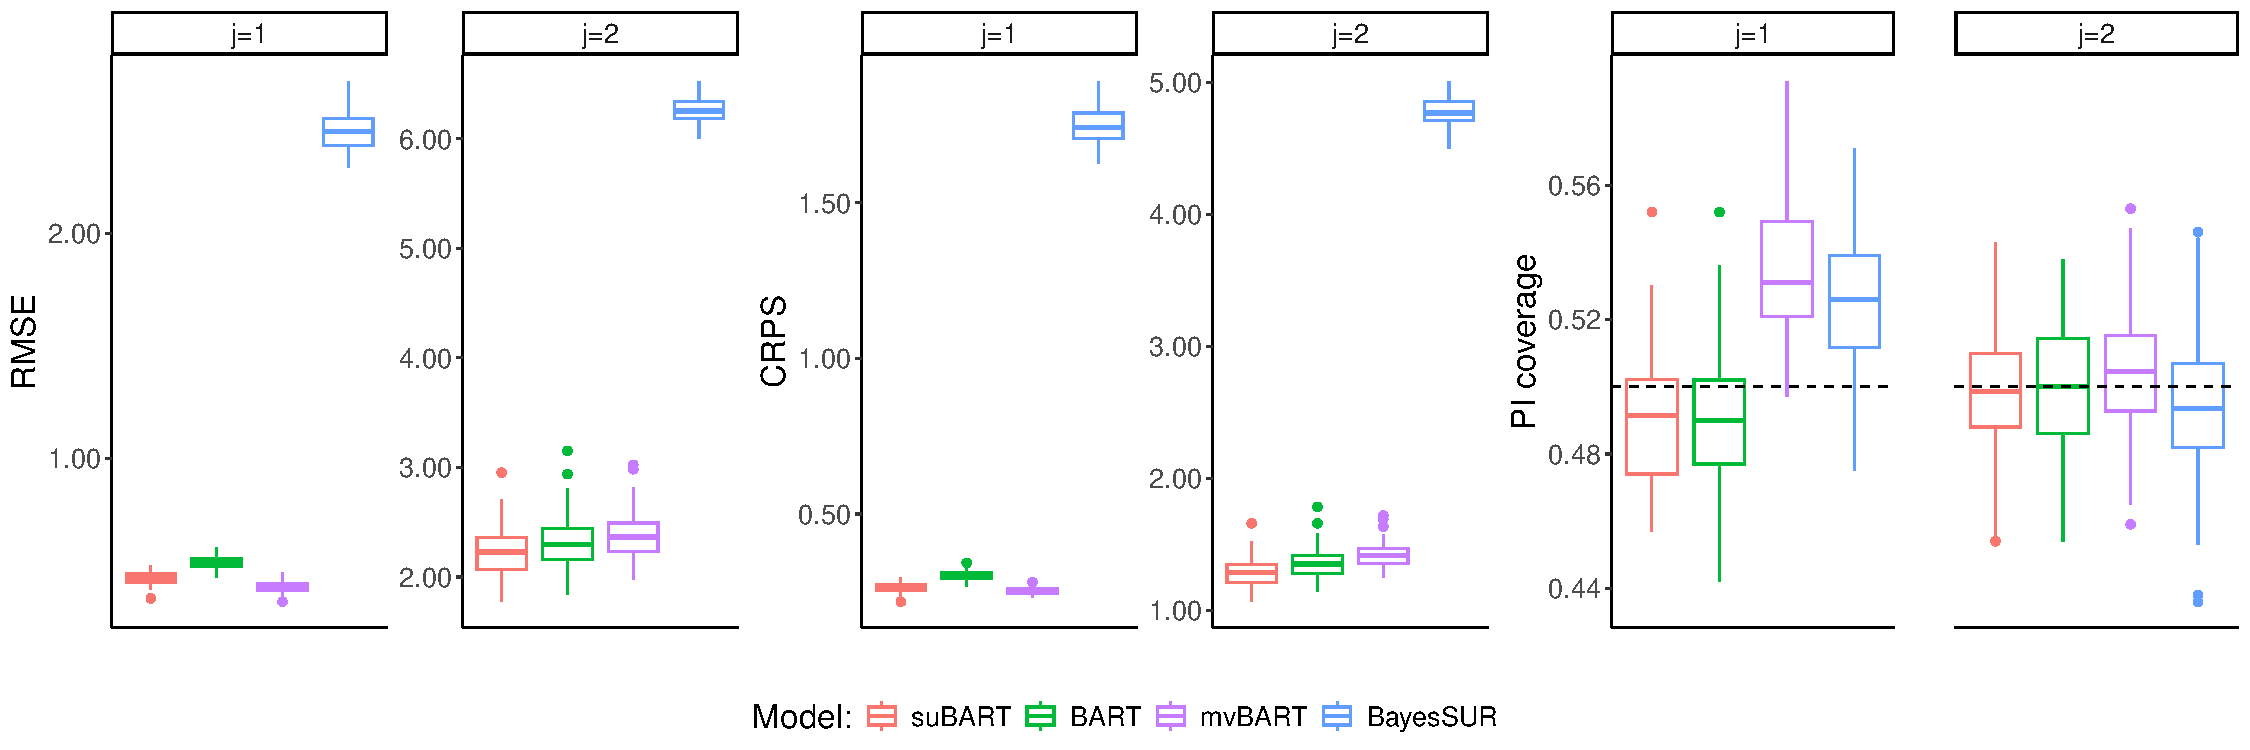
\includegraphics[width=\textwidth]{figures/friedman1_regression_1000_2.pdf}
    \caption{Simulation results for Friedman \#1 under the suBART, BART, mvBART, and BayesSUR models (from left to right) with $n_{\operatorname{train}} = n_{\operatorname{test}}=1000 $ and $d = 2$.}
    \label{fig:sim_reg_friedman_one_1000_2d}
\end{figure}%
\begin{figure}[H]
    \centering
    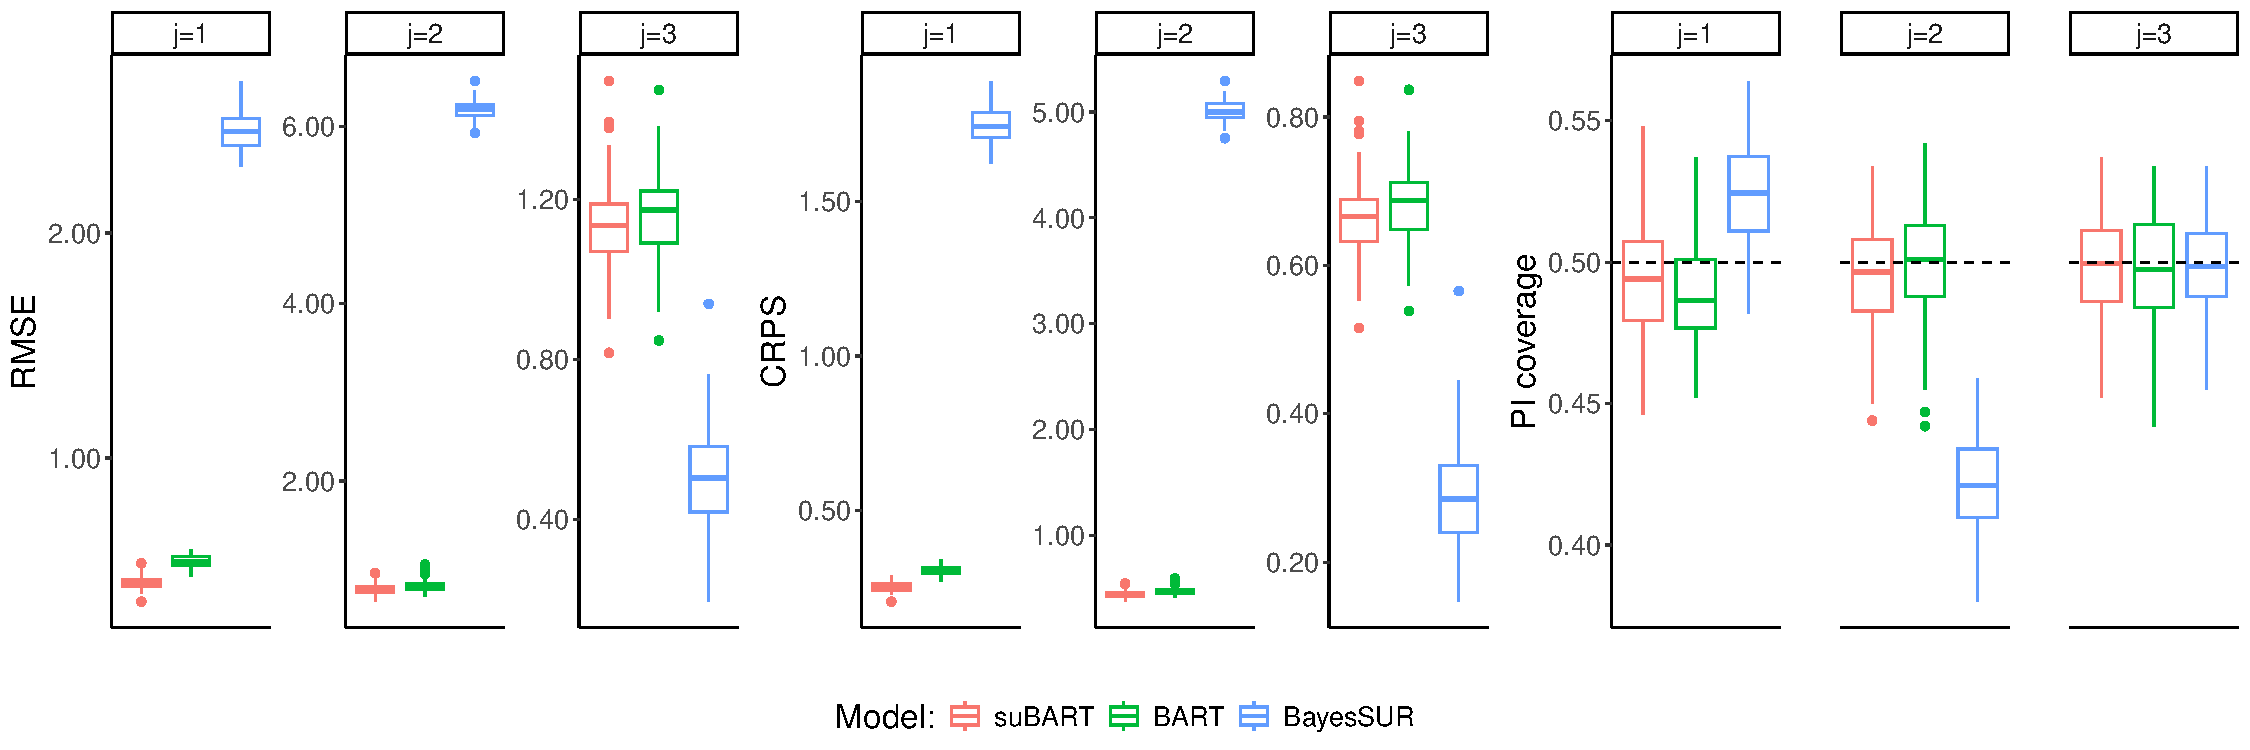
\includegraphics[width=\textwidth]{figures/friedman1_regression_1000_3.pdf}
    \caption{Simulation results for Friedman \#1 under the suBART, BART, and BayesSUR models (from left to right) with $n_{\operatorname{train}} = n_{\operatorname{test}}=1000 $ and $d = 3$.}
    \label{fig:sim_reg_friedman_one_1000_3d}
\end{figure}%
\indent Figure \ref{fig:sim_reg_friedman_one_1000_2d} shows that all methods exhibit reasonable coverage rates for the prediction intervals when $d=2$, except for the first outcome where the coverage is notably high for both mvBART and BayesSUR. Figure \ref{fig:sim_reg_friedman_one_1000_3d} also shows satisfactory coverage for both suBART and mvBART, while the coverage under BayesSUR is only close to the nominal rate when $j = 3$, which is again due to the linearity of this response. It is also vital, for proper uncertainty quantification, to correctly estimate the elements of the matrix $\boldsymbol{\Sigma}$. 
Table \ref{tab:sim_corr_fried_one_combined_1000} gives the RMSE and coverage rates of $50\%$ credible intervals  for all correlation  parameters  $\rho_{jk}$ 
provided by suBART, mvBART, and BayesSUR. Standard deviation parameters $\sigma_j$ are also given, where applicable. Notably, correlations are not provided for the BART model as it assumes independence  (i.e., $\rho_{jk}= 0\:\forall\:j\ne k$), and the mvBART estimates are provided only when $d=2$, due to the aforementioned limitations of the \texttt{skewBART} package.  It is clear from the results that suBART outperforms all competing models in terms of coverage, demonstrating its superior ability to estimate correlation structures. The coverage values of zero for BayesSUR are particularly notable and suggest an inability to accurately estimate correlations when  assuming linear regressions for non-linear responses. In terms of RMSE, suBART is superior to BART and BayesSUR and comparable to mvBART, albeit only in the $d=2$ setting.
\begin{table}[H] 
\small
\centering
\caption{RMSE and coverage of a $50\%$ CI for $\sigma_k$ and ${\rho}_{jk}$  for Friedman \#1 with $n_{\operatorname{train}} = n_{\operatorname{test}} = 1000$.}
\setlength{\tabcolsep}{3.5pt}
\label{tab:sim_corr_fried_one_combined_1000}
\begin{tabular}{llcccccccc}
\hline
\small
&& \multicolumn{4}{c}{\textbf{RMSE}} & \multicolumn{4}{c}{\textbf{CI coverage}} \\
&& \textbf{suBART} & \textbf{BART} & \textbf{mvBART} & \textbf{BayesSUR} & \textbf{suBART} & \textbf{BART} & \textbf{mvBART} & \textbf{BayesSUR} \\
\hline
\multirow{3}{*}{$d=2$} & {$\sigma_1$} & $0.02$ & $0.03$ & $0.03$ & $1.62$ & $0.43$ & $0.26$ & $0.31$ & $0.00$ \\
&{$\sigma_2$} & $0.27$ & $0.33$ & $0.35$ & $1.78$ & $0.32$ & $0.24$ & $0.17$ & $0.00$ \\
&{$\rho_{12}$} & $0.02$ & --- & $0.01$ & $0.31$ & $0.38$ & --- & $0.60$ & $0.00$ \\ 
\hline
\multirow{6}{*}{$d=3$} & {$\sigma_1$} & $0.02$ & $0.04$ & --- & $1.62$ & $0.46$ & $0.28$ & --- & $0.00$ \\
&{$\sigma_2$} & $0.07$ & $0.11$ & --- & $4.15$ & $0.34$ & $0.11$ & --- & $0.00$ \\
&{$\sigma_3$} & $0.18$ & $0.19$ & --- & $0.10$ & $0.25$ & $0.22$ & --- & $0.41$ \\
&{$\rho_{12}$} & $0.01$ & --- & --- & $0.34$ & $0.39$ & --- & --- & $0.00$ \\ 
&{$\rho_{13}$} & $0.02$ & --- & --- & $0.31$ & $0.45$ & --- & --- & $0.00$ \\
&{$\rho_{23}$} & $0.03$ & --- & --- & $0.16$ & $0.50$ & --- & --- & $0.00$ \\ 
\end{tabular}
\end{table}%

\subsection{Binary response experiments}\label{sec:sim_binary}

The experiments for binary responses are aligned with those from Section \ref{sec:sim_continuous}, wherein different sample sizes of $ n_{\operatorname{train}} = n_{\operatorname{test}} = \{250, 500, 1000
\}$ are used for the training and test sets, respectively. The simulation of the latent variables $z^{(j)}$ is described by the system of equations below. Other than when $j=3$, the values of the latent variables are non-linear functions. Recall that correlated noise $(\varepsilon_i^{(1)}, \ldots, \varepsilon_i^{(d)})^\top \sim \operatorname{MVN}_{d}(\mathbf{0}_d, \boldsymbol{\Sigma})$ is subsequently added to the $d$-dimensional latent variable and that the generating process for each binary response follows Equation \eqref{eq:latent_z} thereafter. As the generative model is invariant to the values of the variances \citep{chib1998analysis}, we set them to $1$ for convenience, while the true correlations are set to the same values used in Section \ref{sec:sim_continuous}.\smallskip

\noindent\textbf{Friedman \#2}:
\begin{align*}
x_{i}^{(1)}, \ldots, x_{i}^{(10)} &\overset{\mathrm{iid}}{\sim} \operatorname{Uniform}(0, 1), &
z_{i}^{(1)} &= \sin(x_{i}^{(1)} x_{i}^{(2)} \pi) + {x_{i}^{(3)}}^{3}, \\
z_{i}^{(2)} &= -1 + 2x_{i}^{(1)}x_{i}^{(4)} +e^{x_{i}^{(5)}},&
z_{i}^{(3)} &= 0.5(x_{i}^{(2)} +  x_{i}^{(4)}) + x_{i}^{(5)}.
\end{align*}
\indent The models evaluated for these experiments are the probit suBART and probit extensions of the standard BART and BayesSUR. Since the \texttt{skewBART} software does not offer a probit implementation of the model, for any dimensionality, the mvBART model is excluded. 
We persist in evaluating settings with varying dimension $d=\{2,3\}$ with the $d=2$ setting again comprising the first two responses.
The results for $d=3$, with $n_{\operatorname{train}}=n_{\operatorname{test}}=1000$, are summarised in 
Figure \ref{fig:sim_class_friedman_one_1000_3d} and  are consistent with the findings from Section \ref{sec:sim_continuous}. When logarithmic loss and ACC are considered as metrics for evaluating predictive performance, suBART either exhibits superior results or comparable averages. Both tree-based models outperform Bayesian SUR, with the exception of the linear third response in the $d=3$ setting, as per the continuous-outcome simulation experiments in Section \ref{sec:sim_continuous}.

Regarding calibration, it is evident that suBART and BART are satisfactory across all scenarios, showing coverage rates close to the nominal value. On the other hand, due to the inherent linearity of BayesSUR, its calibration performance is notably poorer, though the third linear response in Figure \ref{fig:sim_class_friedman_one_1000_3d} is again an exception in this regard, as per Section \ref{sec:sim_continuous}. 

Finally, the results regarding the estimation of the correlation parameters $\rho_{jk}$ associated with binary responses when $n_{\operatorname{train}}=1000$ are presented in Table \ref{tab:sim_corr_class_fried_one_combined_1000}, which reports the corresponding RMSE and CI coverage metrics. As BART assumes independent errors, it is excluded from these results. Overall, these results are consistent with Table \ref{tab:sim_corr_fried_one_combined_1000} in clearly demonstrating superior performance for suBART in terms of 
estimating correlation structures.
\begin{figure}[H]
    \centering
    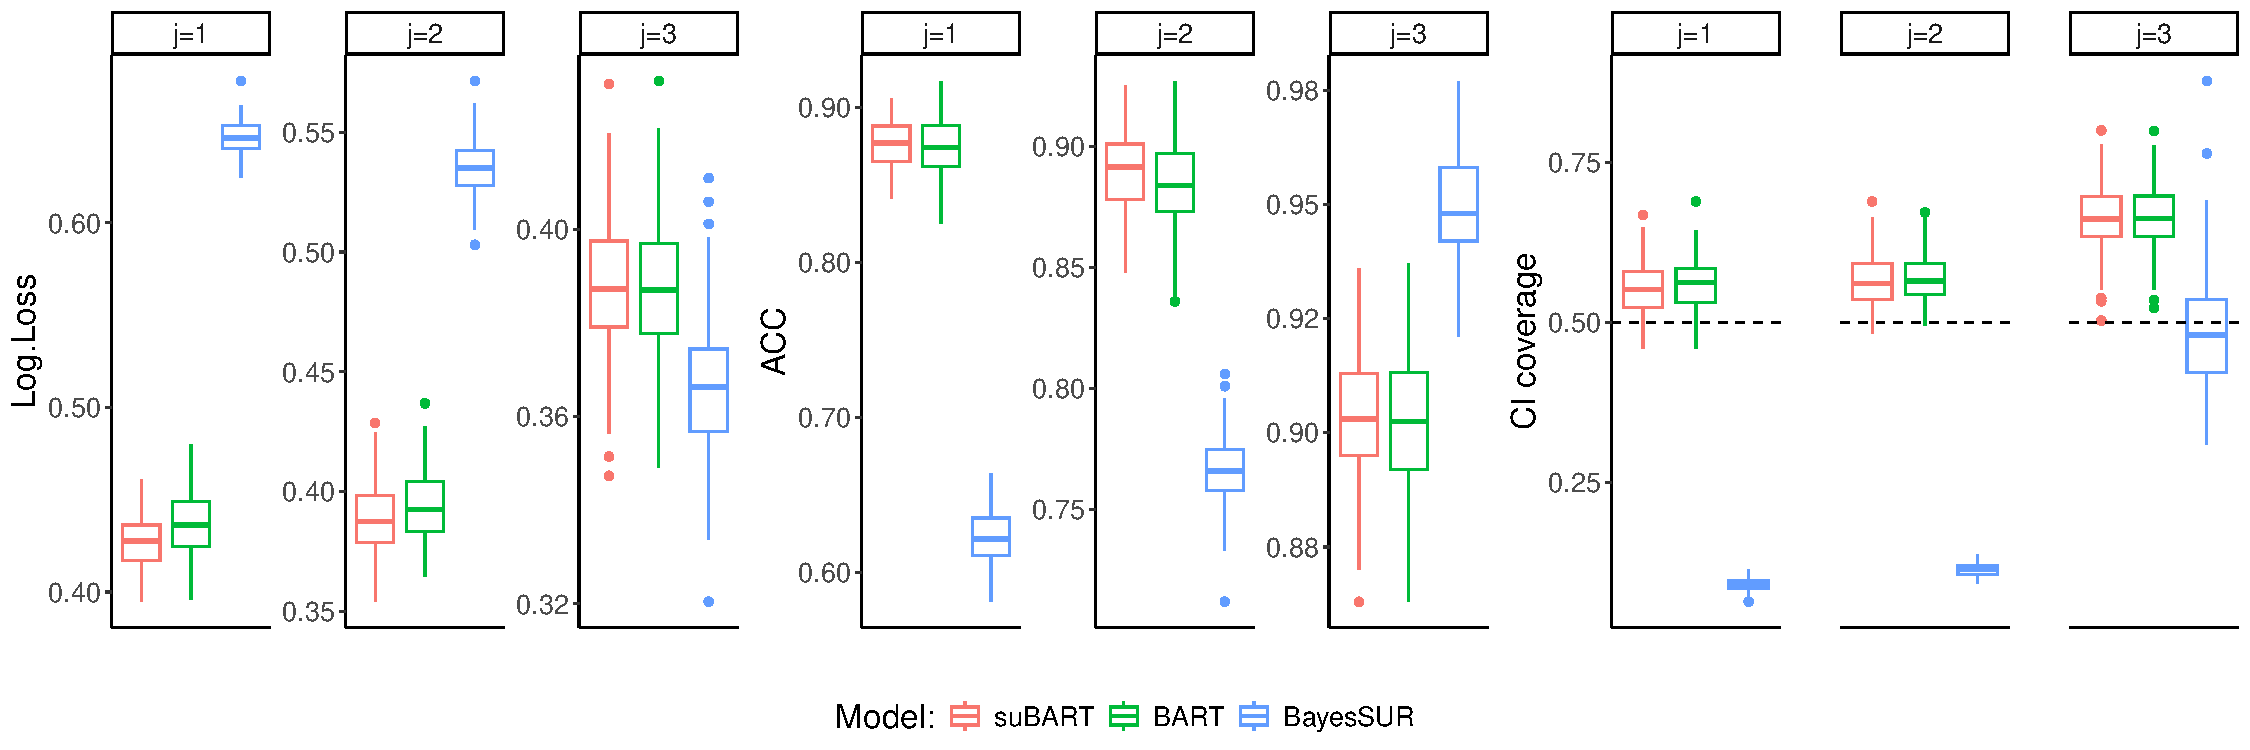
\includegraphics[width=\textwidth]{figures/friedman1_classification_1000_3.pdf}
    \caption{Simulation results for Friedman \#2 under the suBART, BART, and BayesSUR models (from left to right) with $n_{\operatorname{train}} = n_{\operatorname{test}}=1000 $ and $d = 3$.}
    \label{fig:sim_class_friedman_one_1000_3d}
\end{figure}\vspace{-2em}%
\begin{table}[H]
\centering
\caption{RMSE and coverage of a $50\%$ CI for ${\rho}_{jk}$ for Friedman \#2 with $n_{\operatorname{train}} = n_{\operatorname{test}} = 1000$.}
\label{tab:sim_corr_class_fried_one_combined_1000}
\begin{tabular}{llcccccc}
\hline
\small
& & \multicolumn{2}{c}{\textbf{RMSE}} & \multicolumn{2}{c}{\textbf{CI coverage}} \\
& & \textbf{suBART} & \textbf{BayesSUR} & \textbf{suBART} & \textbf{BayesSUR} \\
\hline
$d=2$ & {$\rho_{12}$} & $0.04$ & $0.24$ & $0.39$ & $0.00$ \\ 
\hline
\multirow{3}{*}{$d=3$} & {$\rho_{12}$} & $0.04$ & $0.26$ & $0.44$ & $0.00$ \\
&{$\rho_{13}$} & $0.05$ & $0.09$ & $0.41$ & $0.00$ \\
&{$\rho_{23}$} & $0.05$ & $0.06$ & $0.49$ & $0.00$ \\
\hline
\end{tabular}
\end{table}

\section{Analyses of the TTCM data}\label{sec:case_study}

We now apply the continuous suBART model to the TTCM data from \citet{wiertsema2019cost} introduced in Section \ref{sec:application}. In Section \ref{sec:TTCM_sim}, we apply various models to data created through simulation using the baseline covariates contained in the TTCM data. 
As the true treatment effects are known, this will allow us to evaluate how well each model estimates them. Subsequently, we apply the same models to the full dataset from the TTCM study in Section \ref{sec:TTCM_real_V2}, and compare the results. In each case, we use the same models, software implementations, and priors as in Section \ref{sec:sim_continuous}. Following \citet{wiertsema2019cost}, we specify neither interaction effects nor non-linear terms in the linear predictors for BayesSUR, owing to the difficulties of pre-specifying appropriate functional forms and conducting model selection in the presence of a large number of covariates. In any case, \citet{dorie2019automated} found that linear models perform poorly in causal settings even with interactions, polynomial terms, and regularisation to avoid overfitting. Conversely, BART-based methods are well-equipped to automatically capture low-order interactions and non-linearities \citep{rockova2020semi,rockova2020posterior}.

In addition, we evaluate each model again with the set of predictors augmented using point estimates of the propensity scores obtained via probit BART. This procedure is inspired by the univariate ps-BART method proposed by \citet{hahn2020bayesian}, which induces a covariate-dependent prior on the regression function. This step 
can substantially reduce bias due to regularisation-induced confounding, thereby making the models less prone to attributing the effect of confounders to the treatment variable and yielding results which are more robust to model misspecification \citep{li2023bayesian}\footnote{
There is some conceptual disagreement as to whether to merely include point estimates of the propensity scores among the covariates or to condition on the propensity scores.
\citet[Section~8.3]{hahn2020bayesian} argue convincingly in favour of the former. Our adoption of this approach is also well-supported by the extensive simulations of \citet{dorie2019automated}, which show that ps-BART performs well from a frequentist perspective.
For an opposing viewpoint arguing for joint modelling of the outcomes and treatment indicators, see \citet[Section~5]{li2023bayesian}.}. We first estimate propensity scores for each patient through probit BART, which give the probability that a patient received treatment $1$, conditional on their baseline characteristics, and then add the posterior mean propensity score estimates to the set of predictors $\mathbf{x}_i$ used to estimate the conditional expectations $\mathbb{E}\lbrack c_i\given t_i, \mathbf{x}_i\rbrack$ and $\mathbb{E}\lbrack q_i\given t_i, \mathbf{x}_i\rbrack$ via the chosen model. 
Thus, we expand the comparison to include what we refer to as ps-suBART, ps-mvBART, and ps-BayesSUR, which are straightforward adaptations of the univariate ps-BART method. Although the use of BART-based propensity scores in conjunction with linear SUR deviates from usual practice in the applied health economics literature, we nonetheless use the same set of propensity scores estimated via probit BART for each method, in order to ensure the comparison is fair in this regard. Expanding the comparison to include versions of each method with and without propensity scores will help to establish the extent to which differences in results are attributable to differences in model specification or due to the inclusion of propensity scores.

Given that there are several unordered categorical covariates with more than two levels in the TTCM dataset --- \textit{fracture region}, \textit{medical history}, and \textit{trauma type} --- such variables require particular attention. With probit BART (when estimating the propensity scores) and suBART, we treat such predictors by adapting the method of ordering categories proposed by \citet{breiman1984classification}.
More specifically, whenever such a variable is split on, we order the levels according to the mean values of the partial residuals and then treat the reordered variable in the same way as a continuous variable. This approach makes the tree-growing process more effective by allowing splitting rules which group multiple levels and can reduce the risk of overfitting by allowing for shallower trees. By contrast, both mvBART and BayesSUR accommodate these predictors as dummy variables.

\subsection{CEA simulation experiments}\label{sec:TTCM_sim}
In this section, we present the results of a simulation experiment based on the TTCM data. We keep the baseline covariates fixed and define generative functions for the potential outcomes and propensity scores. We then simulate treatments and outcomes for each patient and use all six previously discussed models to estimate the treatment effects and $\operatorname{INB}_\lambda$ at representative values of $\lambda=20\mathrm{k}$ and $\lambda=50\mathrm{k}$, where $\lambda=20\mathrm{k}$ corresponds to €20,000. These threshold values are commonly used for determining whether an intervention represents value for money in the CEA literature \citep{drummond2015methods,gabrio2019bayesian}.
By repeating this procedure $1000$ times, we investigate how well each method performs at recovering the true parameters used in the simulation. We summarise the performance in terms of bias, standard deviation (SD), and RMSE, all evaluated using the posterior mean as a point estimate. We also include the coverage rates of $50\%$ credible intervals (CI coverage) and their average width (CI width). 

Our data-generating process, given by 
\begin{align*}
\mu_c(\mathbf{x}_i) &= 2000 + 500x^{(1)}_i -200x^{(2)}_i + 500x^{(4)}_i,&\mu_q(\mathbf{x}_i) &= 0.5 + 0.2(x^{(3)}_i + 1)\sin(x^{(1)}_i), \\
\tau_c(\mathbf{x}_i) &= 500,&\tau_q(\mathbf{x}_i) &= -0.1 + 0.1\exp(-x^{(5)}_i), \\
c_i &= \mu_c(\mathbf{x}_i) + t_i \times \tau_c(\mathbf{x}_i) + \varepsilon^{(1)}_i,  
&q_i &= \mu_q(\mathbf{x}_i) + t_i \times \tau_q(\mathbf{x}_i) + \varepsilon^{(2)}_i,
\end{align*}
\[\begin{pmatrix}  \varepsilon_i^{(1)} \\ \varepsilon_i^{(2)} \end{pmatrix} \sim \operatorname{MVN}_2 \left( \begin{pmatrix}  0 \\ 0 \end{pmatrix} , \begin{pmatrix}  500^2 & -0.25 \times 500 \times 0.05 \\ -0.25 \times 500 \times 0.05 & 0.05^2 \end{pmatrix}\right),\]
uses the \textit{age}, \textit{education level}, \textit{gender}, \textit{surgery}, and \textit{TTO} covariates from the TTCM data, which we refer to as $x^{(1)}_i, \dots, x^{(5)}$, respectively. This design is inspired by the simulation experiments in \citet{hill2011bayesian} and \citet{hahn2020bayesian}, but there are also important novelties. There is first the CEA setting with two correlated outcomes, for which the suBART model was developed. We also use somewhat larger variances for the error terms in the simulation (not necessarily in absolute terms, but relative to the variation in $\mathbb{E}\lbrack c_i\given \mathbf{x}_i\rbrack$ and  $\mathbb{E}\lbrack q_i\given \mathbf{x}_i\rbrack$). In our experience, this is more reflective of real cost-effectiveness datasets. 
The continuous covariates are normalised prior to generating the outcomes. For the sake of clarity, we introduce the additional notation $\mu_c(\mathbf{x}_i) \coloneqq \mathbb{E}\left\lbrack c_i(0)\given \mathbf{x}_i\right\rbrack$ and $\tau_c(\mathbf{x}_i) \coloneqq \mathbb{E}\left\lbrack c_i(1)\given \mathbf{x}_i\right\rbrack - \mathbb{E}\left\lbrack c_i(0)\given \mathbf{x}_i\right\rbrack$, adopt analogous definitions for $q$, and let $\overline{\mu_q(\mathbf{x}_i)}$ and $\operatorname{sd}(\mu_q(\mathbf{x}_i))$ denote the corresponding sample mean and standard deviation, respectively.

The coefficients are chosen such that the simulated outcomes are reflective of values typically observed in CEA data. We emphasise that the data-generating process is linear for $c_i$ and non-linear for $q_i$. In particular, the treatment effect $\tau_q(\mathbf{x}_i)$ is heterogeneous, given its dependence on the \textit{TTO} covariate, while $\tau_c(\mathbf{x}_i)$ is constant. 
These settings imply true values for $\Delta_c$, $\Delta_q$, $\operatorname{INB}_{20\mathrm{k}}$, and $\operatorname{INB}_{50\mathrm{k}}$ of $500$, $0.0399$, $299.24$, and $1489.10$, respectively. We specify a negative correlation of $-0.25$ for the errors to model a common occurrence in CEA studies: patients who report lower well-being also have higher associated costs \citep{glick2014economic}.
The results of additional experiments using correlation values of $0$ and $-0.5$ --- considering only ps-suBART and independent BART models --- are deferred to Appendix~A.

We further define the propensity scores $\pi_i \coloneqq \Pr(t_i = 1 \given \mathbf{x}_i)$ as follows:
\begin{equation}
\pi_i = 0.9 \Phi\left(-0.5 + x^{(4)}_i -1.5\left(\frac{\mu_q(\mathbf{x}_i) - \overline{\mu_q(\mathbf{x}_i)}}{\operatorname{sd}(\mu_q(\mathbf{x}_i))}\right)\right) + 0.05.\label{eq:ps_dgp}
\end{equation}
By design, the propensity scores are strongly dependent on $\mu_q(\mathbf{x}_i)$, which is the expected health outcome under treatment $0$. This is an example of \textit{targeted selection} \citep{hahn2020bayesian}, which induces strong confounding with respect to the outcome $q_i$, and reflects how treatments are assigned in reality: patients expected to have a bad outcome under treatment $0$ are more likely to be given treatment $1$ by medical professionals. Further confounding with respect to $c_i$ arises by including dependence on the \textit{surgery} covariate, on which $\mu_c(\mathbf{x}_i)$ also depends, in Equation \eqref{eq:ps_dgp}. The coefficients are chosen to ensure roughly balanced sample sizes for the two treatment groups.

Table \ref{tab:results_Delta_cq} presents the performance metrics (under all six models, across $1000$ simulation replications) for $\Delta_c$ and $\Delta_q$, while Table \ref{tab:results_INB} reports the corresponding results for $\operatorname{INB}_\lambda$. We see that including propensity scores generally leads to smaller bias and improved coverage rates, while slightly increasing the SD of the estimates. Including propensity scores also lowers the RMSE in all but one case while increasing the average CI width for all methods. Across all estimands, the intervals from BayesSUR are wider than those from mvBART, which in turn are wider than those from suBART, with or without propensity scores. For $\Delta_c$, the BayesSUR models have the smallest bias, which is expected given the linearity of $\mu_c(\mathbf{x}_i)$ in the data-generating process. For $\Delta_q$, ps-suBART exhibits the lowest bias by far, and also the lowest RMSE by a reasonable margin. BayesSUR exhibits substantial bias for $\Delta_q$, although this is mitigated through the inclusion of propensity scores. For $\operatorname{INB}_\lambda$, ps-suBART's superiority in terms of bias, RMSE, and coverage notably holds at both $\lambda=20\mathrm{k}$ and $\lambda=50\mathrm{k}$.

The results also show that the non-linear BART models perform only slightly worse than linear BayesSUR when the conditional expectation is actually linear ($\Delta_c$ in Table \ref{tab:results_Delta_cq}), and much better when it is non-linear ($\Delta_q$ in Table \ref{tab:results_Delta_cq}). The subpar performance of SUR in the second case can be improved significantly by the inclusion of propensity scores, which seem to absorb much of the non-linearity, although we emphasise that this is a somewhat unnatural model which is unlikely to be used by anyone in practice; if we estimate propensity scores through a non-linear model, it would seem appropriate to also use a non-linear outcome model. Comparing ps-suBART and ps-mvBART specifically, we see a better performance from ps-suBART across all estimands and metrics. Overall, ps-suBART exhibits the smallest bias and RMSE, while also being competitive in terms of interval width and coverage.
\begin{table}[H]
\caption{Performance metrics for $\Delta_c$ and $\Delta_q$, evaluated over $1000$ simulation replications. \label{tab:results_Delta_cq}}
\setlength{\tabcolsep}{2.76pt}
\begin{tabular}{lrrrrrrrrrrr}
\multirow{2}{*}{\textbf{Model}} &\multicolumn{5}{c}{$\mathbf{\Delta_c}$}&\multicolumn{5}{c}{$\mathbf{\Delta_q}$}\\
\cline{2-11}
 & Bias & SD & RMSE & CI coverage & CI width & Bias & SD & RMSE & CI coverage & CI width \\
\hline
\textbf{ps-suBART} & $-60$& $118$& $132$& $0.423$& $159$& $-0.0041$& $0.0160$& $0.0166$& $0.475$& $0.0207$ \\
\textbf{suBART} & $-101$& $113$& $151$& $0.358$& $150$& $-0.0115$& $0.0155$& $0.0193$& $0.348$& $0.0191$\\
\textbf{ps-mvBART} & $-93$& $109$& $144$& $0.404$& $160$& $-0.0088$& $0.0161$& $0.0184$& $0.522$& $0.0251$\\
\textbf{mvBART} & $-110$& $107$& $154$& $0.343$& $154$& $-0.0162$& $0.0157$& $0.0225$& $0.371$& $0.0236$\\
\textbf{ps-BayesSUR} & $14$& $141$& $142$& $0.493$& $189$& $-0.0056$& $0.0230$& $0.0237$& $0.592$& $0.0385$\\
\textbf{BayesSUR} & $4$& $125$& $125$& $0.478$& $167$& $-0.0574$& $0.0227$& $0.0617$& $0.039$& $0.0360$
\end{tabular}
\end{table}
\vspace{-2em}
\begin{table}[H]
\caption{Performance metrics for $\operatorname{INB}_\lambda$ with $\lambda = 20\mathrm{k}$ and $\lambda=50\mathrm{k}$, evaluated over $1000$ simulation replications. \label{tab:results_INB}}
\setlength{\tabcolsep}{3.21pt}
\begin{tabular}{lrrrrrrrrrrr}
\multirow{2}{*}{\textbf{Model}} &\multicolumn{5}{c}{$\textbf{INB}_{\mathbf{20k}}$}&\multicolumn{5}{c}{$\textbf{INB}_{\mathbf{50k}}$}\\
\cline{2-11}
 & Bias & SD & RMSE & CI coverage & CI width & Bias & SD & RMSE & CI coverage & CI width \\
\hline
\textbf{ps-suBART} &$-22$& $353$& $354$& $0.466$& $467$& $-146$ & $823$& $836$& $0.473$& $1071$ \\
\textbf{suBART} & $-130$& $342$& $366$& $0.452$& $433$& $-475$& $795$& $926$& $0.392$& $991$\\
\textbf{ps-mvBART} & $-83$& $349$& $359$& $0.560$& $543$& $-349$& $823$& $894$ & $0.527$& $1282$\\
\textbf{mvBART} & $-212$& $341$& $401$& $0.482$& $514$& $-697$& $801$& $1062$& $0.422$& $1208$\\
\textbf{ps-BayesSUR} & $-127$& $501$& $517$& $0.586$& $815$& $-296$& $1180$& $1217$& $0.597$& $1957$\\
\textbf{BayesSUR} & $-1151$& $483$& $1249$& $0.053$& $757$& $-2872$& $1155$& $3096$& $0.042$& $1824$
\end{tabular}
\end{table}

\subsection{Results of the TTCM data analysis}\label{sec:TTCM_real_V2}
Figure \ref{fig:PSplot} shows the distribution of the estimated propensity scores. Although there is some overlap, it is evident that the treatment groups are quite imbalanced with respect to their baseline characteristics and that some form of covariate adjustment is necessary to avoid biased results. As already described, we reevaluate each model with estimated propensity scores included as an additional covariate. In Figure \ref{fig:CEplane_model_comparison} we show highest density regions of kernel density estimates of the posterior distributions of $\Delta_c$ and $\Delta_q$ --- obtained through suBART, mvBART, and BayesSUR, as well as their counterpart models which also incorporate the estimated propensity scores as additional predictors --- in the form of a cost-effectiveness plane 
(CEP; see \citet{gabrio2019bayesian} for more details). 
In general, for both $\Delta_c$ and $\Delta_q$, the centers of the distributions are shifted further away from $0$ and posterior uncertainty is greater when the propensity scores are incorporated. These differences are most pronounced between ps-BayesSUR and BayesSUR. A notable distinction between suBART and BayesSUR is that the latter appears to be more uncertain about $\Delta_q$.
The same applies to the comparison between ps-suBART and ps-BayesSUR.\vspace{-1ex}
\begin{figure}[H]
    \centering
    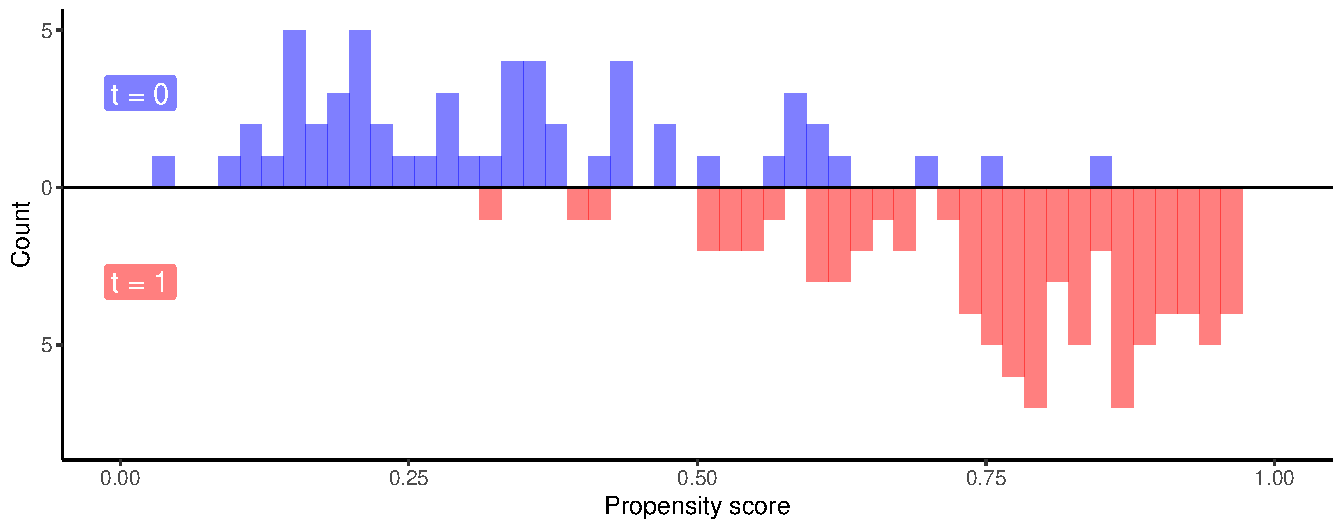
\includegraphics[width=\textwidth]{figures/PSplot.pdf}
    \caption{Propensity scores by treatment group, estimated via probit BART, where $t=0$ corresponds to the control group and $t=1$ denotes the TTCM intervention.}
    \label{fig:PSplot}
\end{figure}%
\begin{figure}[H]
    \centering
    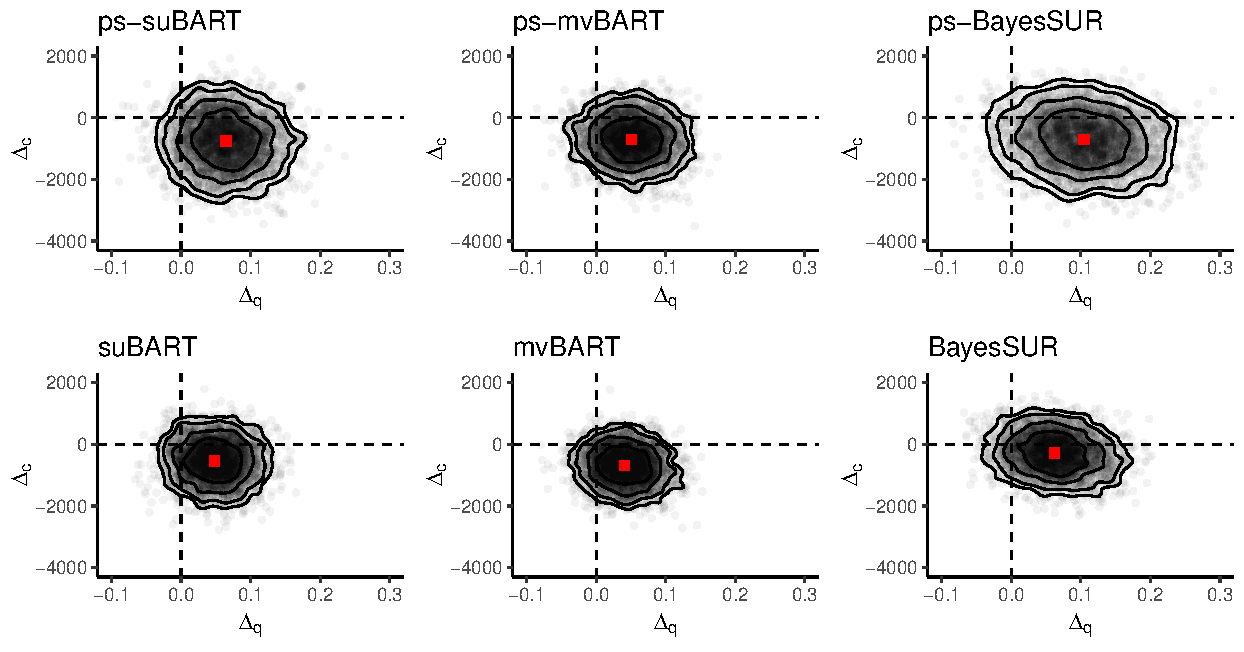
\includegraphics[width=\textwidth]{figures/CEplane_comparison_v11.pdf}
    \caption{CEPs showing highest density regions of kernel density estimates of the posterior distributions of $\Delta_c$ and $\Delta_q$ according to each model. Each point represents an individual draw of $\Delta_c$ and $\Delta_q$. Posterior means are indicated by squares and the contour lines correspond to probability levels of $0.5$, $0.75$, $0.9$, and $0.95$.} 
    \label{fig:CEplane_model_comparison}
\end{figure}\vspace{-1em}%
Table \ref{tab:inb_ci} gives summary statistics for $\Delta_c$, $\Delta_q$, and the INB at the same representative values of $\lambda = 20\mathrm{k}$ and $\lambda=50\mathrm{k}$ adopted in Section \ref{sec:TTCM_sim}. 
We see some considerable differences between ps-suBART and the other methods. This suggests that there may be strong non-linear functional relationships between the covariates and the outcomes and that those relationships may differ for the two outcomes $c_i$ and $q_i$. It thus appears that suBART benefits from relaxing the linearity assumption of BayesSUR, without requiring pre-specification of the functional forms, and also benefits from relaxing mvBART's assumption of a common tree structure. Apart from ps-BayesSUR, the INB values from all models are much lower than those from ps-suBART. For all models, the estimated treatment effects, and $\operatorname{INB}_\lambda$ (at both $\lambda$ values), are consistently larger in absolute value for each method when propensity scores are included. 
Surprisingly, for both $\Delta_q$ and $\operatorname{INB}_\lambda$, ps-BayesSUR produces far higher estimates than all other models.
We recall here that, in Section \ref{sec:TTCM_sim}, the standard error of the $\Delta_q$ estimates was the highest by far for ps-BayesSUR. As this model's estimation of $\Delta_q$ tends to be rather volatile, we are thus inclined to put more faith in the estimates from the other models.\vspace{-1ex}
\begin{table}[H]
\caption{Posterior means (with $95\%$ credible intervals in brackets) for $\Delta_c$, $\Delta_q$, and $\operatorname{INB}_\lambda$ at representative values of $\lambda=20\mathrm{k}$ and $\lambda=50\mathrm{k}$ for each model, with and without the propensity scores.\label{tab:inb_ci}}
\setlength{\tabcolsep}{3.33pt}
\begin{tabular}{lrrrrrrrr}
\textbf{Model} & \multicolumn{2}{c}{$\mathbf{\Delta_c}$}  & \multicolumn{2}{c}{$\mathbf{\Delta_q}$} & \multicolumn{2}{c}{$\mathbf{INB_{20\mathrm{k}}}$}& \multicolumn{2}{c}{$\mathbf{INB_{50\mathrm{k}}}$}\\
\hline
\textbf{ps-suBART}   & $-759$&$\lbrack-2321, 745\rbrack$ & $ 0.064$&  $\lbrack-0.013, 0.147\rbrack$ & $2045$&$\lbrack-217, 4317\rbrack$  &$3975$&$\lbrack-250, 8519\rbrack$  \\
\textbf{suBART}   & $-537$&$\lbrack-1752, 619\rbrack$ & $0.048$&$\lbrack-0.016, 0.114\rbrack$ & $1500$&$\lbrack-338, 3320\rbrack$  &$2943$&$\lbrack-627, 6497\rbrack$  \\
\textbf{ps-mvBART}   & $-706$&$\lbrack-1938, 518\rbrack$ & $0.051$&$\lbrack-0.022, 0.122\rbrack$ & $1717$&$\lbrack-245, 3631\rbrack$ &$3234$&$\lbrack-647, 7054\rbrack$  \\
\textbf{mvBART}   & $-692 $&$\lbrack-1781, 359\rbrack$ & $0.041$&$\lbrack-0.021, 0.104\rbrack$ & $1511$&$\lbrack-162, 3235\rbrack$ &$2740$&$\lbrack-588, 6235\rbrack$  \\
\textbf{ps-BayesSUR} & $-698$&$\lbrack-2253, 795\rbrack$ & $0.104$&$\lbrack-0.007, 0.214\rbrack$  & $2783$&$\lbrack-55, 5646\rbrack$ &$5912$&$\lbrack-80, 11735\rbrack$  \\
\textbf{BayesSUR} & $-286$&$\lbrack-1400, 827\rbrack$ & $0.063$&$\lbrack-0.016, 0.145\rbrack$  & $1537$&$\lbrack-538, 3723\rbrack$ &$3413$&$\lbrack-901, 7959\rbrack$
\end{tabular}
\end{table}\vspace{-1ex}
Figure \ref{fig:CEAC_comparison} shows the probability of cost-effectiveness as a function of $\lambda$, the willingness-to-pay, in the form of a cost-effectiveness acceptability curve \citep[CEAC;][]{lothgren2000definition}. CEACs are an important tool for guiding decisions of which medical interventions to implement. The probabilities are estimated by simply counting all posterior draws for which $\operatorname{INB}_{\lambda} > 0$ and dividing this count by the total number of posterior draws.\vspace{-1ex} 
\begin{figure}[H]
    \centering
    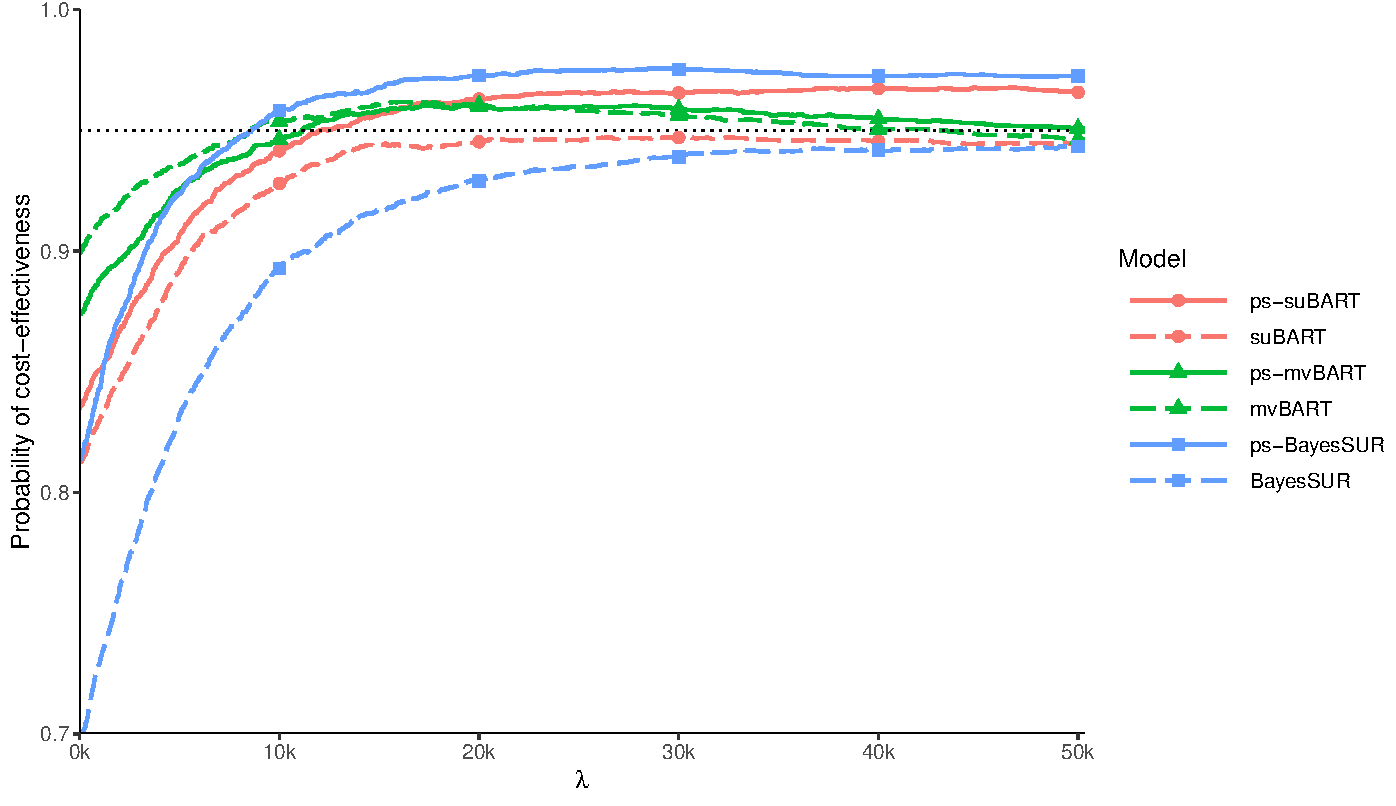
\includegraphics[width=\textwidth]{figures/CEAC_comparison_v6.pdf}
    \caption{CEACs showing probabilities of cost-effectiveness as a function of $\lambda$ for suBART, mvBART, and
    BayesSUR,
    with (solid lines) and without (dashed lines) propensity scores, with a dotted line at the $0.95$ reference level.} 
    \label{fig:CEAC_comparison}
\end{figure}\vspace{-1em}%
For suBART and BayesSUR, including the propensity scores leads to a uniformly higher probability of cost-effectiveness. Hence, these methods give greater certainty to the  conclusion that the treatment is cost-effective. The greatest difference in this regard is observed for BayesSUR. Although mvBART does not exhibit the same effect, all three models involving propensity scores yield a similar insight: if $\lambda$ exceeds a value of around $10\mathrm{k}$, then the probability of cost-effectiveness exceeds $0.95$, which is a commonly used benchmark in CEAs.
We stress, however, that the superiority of any one method cannot be established from these estimated CEACs, as the true $\operatorname{INB}_{\lambda}$ is unknown for all values of $\lambda$. In light of the simulation study based on the TTCM data presented in Section \ref{sec:TTCM_sim}, which demonstrated the superiority of ps-suBART in recovering the true INB, we tend to trust the estimates from this model.

In Appendix~D, we sketch two additional analyses of the TTCM data, which also showcase some additional features of our computational implementation: Appendix~D.1 shows how we can estimate treatment effects for individual patients in the TTCM data, and how they vary depending on the baseline covariates, while Appendix~D.2 shows variable importance plots for suBART, created in much the same way as for the standard BART.

\section{Discussion}\label{sec:conclusion}

This paper introduces the suBART model for multivariate outcomes in order to account for non-linearities and interactions in the SUR framework and address the key limitation of existing multivariate BART approaches which assume a single set of trees, such that the entire response vector is partitioned in the same way by the splitting rules in the ensemble. By modelling each component of the outcome via univariate BART, suBART captures non-linearities and interactions in the relationships between the responses and predictors while allowing for and detecting the different subsets of covariates associated with each response, without enforcing common tree structures. Another defining feature of suBART is that it handles dependencies between the outcomes through correlated error terms. 

We further develop a probit version of the suBART model to handle multivariate binary outcomes. The effectiveness of both versions is demonstrated through extensive simulation experiments in Section \ref{sec:simstudies}. It is shown that the model adequately captures non-linear responses, accurately estimates the covariance structure for multivariate responses, and generally outperforms other tree-based competitors and the Bayesian linear SUR from the points of view of both predictive accuracy and uncertainty quantification. Notably, suBART is consistently superior to the strategy of applying the standard BART model independently to each response, which demonstrates the benefits of modelling the covariance between multivariate response under our suBART framework. Furthermore, the results show that the model exhibits enhanced flexibility compared to its direct multivariate counterpart, mvBART, by allowing the trees for each outcome component to differ rather than imposing common tree structures. This enables a more accurate representation, especially when different outcome components depend on distinct sets of predictors. As a cautionary note, we recall that BayesSUR exhibited competitive performance 
when estimating conditional expectations which merely depend linearly on the predictors.
In situations where linearity can be reasonably assumed for every outcome, BayesSUR would remain a viable alternative to suBART.

The main focus of this paper is the application of suBART within the context of cost-effectiveness analysis, a setting in healthcare research where it is of interest to jointly estimate the healthcare costs and the health-related quality of life associated with two or more treatment options. Throughout Section \ref{sec:case_study}, we find some remarkable differences, both for the additional simulation experiment in Section \ref{sec:TTCM_sim} and the main application in Section \ref{sec:TTCM_real_V2}, depending on the particular method used for analysing the TTCM data. It is, of course, expected to see large differences between linear SUR and the two BART-based models, given the very different model assumptions. The significant differences between suBART and mvBART are arguably even more interesting, and suggest to us that mvBART's assumption of a shared tree structure is a significant one, which can strongly impact the results. 
Unlike mvBART, suBART can accommodate data where the dependence on $\mathbf{X}$ is very different for different components of the outcome vector. In the CEA context, this applies particularly in situations where factors which govern the costs are unrelated to the quality of life, and \textit{vice versa}. Such situations do occur in practice: when investigating the effect of total knee replacement, \citet{dakin2012rationing} found that the patient's sex was a strong predictor of healthcare costs yet had no measurable relationship with quality of life, while the exact opposite was true for the patient's age. On the other hand, a shared tree structure may lead to estimates which are more precise, in the sense of having a smaller variance, since there are more data available to inform the tree structure. \citet{um2023bayesian} claim this as an advantage of their method. Our results are somewhat inconclusive in this respect: when estimating the MATE on the costs, mvBART exhibits slightly smaller standard deviation than suBART, while both methods are similar in this respect for the quality of life and the INB. Finally, these experiments also show that allowing for correlated error terms is key: running independent BART models implicitly assumes that $\boldsymbol{\Sigma}$ is diagonal, which has been shown to harm performance (see Appendix~A).

According to our simulation experiment in Section \ref{sec:TTCM_sim}, which was explicitly based on the TTCM data, the ps-suBART model demonstrates superior performance over all competing methodologies. Recall that this extension includes propensity scores estimated via BART as an additional predictor in suBART. 
We are hence inclined to believe that the ps-suBART results are the most reliable for the real TTCM application. More generally, we consider the ps-suBART model to be a natural adaptation of the univariate BART approach and expect it to be an especially useful tool in the analysis of cost-effectiveness data.

Despite the extensive array of comparisons and scenarios and the additional insights gleaned by suBART in the CEA setting, there remains ample opportunity for further exploration of various extensions to suBART. We delineate some of these possibilities below in light of limitations identified in the simulation experiments and the real data application.
\begin{itemize}[wide]
    \item Many extensions to the BART model for univariate outcomes have been proposed in the literature. It may be of interest to extend suBART in similar ways, for other applications beyond the TTCM data considered here. For example, methods designed to address the inherent discontinuity and lack of smoothness of regression trees based on sums of piecewise constants \citep[e.g.][]{linero2018bayesian, prado2021bayesian, maia2024gp} could be adapted to suBART. Another extension, which we did not adopt here due to the relatively small number of covariates in the TTCM data, is the sparsity-inducing Dirichlet prior on the splitting probabilities \citep{linero2018highdim}, which could allow suBART to be used in high-dimensional settings. However, it remains to be seen how such extensions would perform in causal settings. Furthermore, embedding these and other BART extensions in the suBART framework could present some computational challenges.
    \item Our simulation experiments comprehensively demonstrated suBART's superiority in capturing non-linear relationships. However, BayesSUR was slightly preferable when the response was generated by a simple linear function. In light of this, we can also envision a hybrid approach, whereby some outcomes would be modelled nonparametrically via BART, and others parametrically via linear models. We stress that this would differ from existing approaches referred to in the literature as semi-parametric BART \citep[e.g.][]{zeldow2019semiparametric,deshpande2020,prado2025accounting}, where each response is modelled by a combination of parametric and non-parametric forms. While such semi-parametric extensions of suBART would also be of interest, we are describing here a model which would instead assign either a BART model or a linear predictor to each outcome. In situations where linearity holds for one outcome but not for others (such as the one presented in Section \ref{sec:TTCM_sim}), such a model may be preferable to both suBART and linear SUR. 
    However, a practical challenge of this hybrid model is that it would require strong prior beliefs about which outcomes should explicitly be specified as having simpler, linear functional forms. 
    \item Accounting for heteroscedasticity in traditional, linear SUR models has been a common challenge in the literature \citep{afolayan2018efficiency}. As suBART represents an effective alternative to SUR, the extension proposed by \citet{pratola2020heteroscedastic} to accommodate heteroscedasticity within BART could be adapted to the suBART setting to address cases where the homoscedasticity assumption is invalid. However, it is important to note that the approach of \citet{pratola2020heteroscedastic} has yet to be extended beyond scalar variance estimation.
    \item The proposed suBART accommodates two types of multivariate outcomes: all continuous and all binary. We stress, however, that this flexibility is exclusive and does not apply to both types simultaneously. Previous works in the literature have used Bayesian frameworks to handle responses of mixed type \citep[e.g.][]{flexible2014papa, zhang2015bayesprobit, bayesianmix20216tony}, which could potentially be generalised within our suBART approach, particularly given that trading off treatment costs against binary outcomes (e.g., cancer remission) is often of interest in other healthcare applications.
    \item The ps-suBART model used in our analysis of the TTCM data builds on the ps-BART model of \citet{hahn2020bayesian}, who also propose the related Bayesian causal forest (BCF) method. The authors and their discussants found the performance of ps-BART and BCF to be similar overall, with each method improving on the other in some settings. One advantage of BCF is the ability to explicitly specify a prior on the amount of treatment effect heterogeneity, while this prior is left implicit in ps-BART. The drawback of this flexibility is that prior specification is more complex in BCF, and it is harder to find reasonable default choices which suit a variety of settings. The computational demands of BCF are also greater than those of BART. Both aspects would become even more challenging in the SUR setting with multiple outcomes. Nonetheless, embedding BCF in the SUR framework could present a promising alternative to the multivariate generalisation of BCF proposed by \citet{mcjames2024bayesian}, which is analogous to the multivariate BART model of \citet{um2023bayesian}.
    \item CEAs are sometimes conducted with more than two treatment options of interest. This is conceptually similar to the two-treatments setting presented in the TTCM application. We refer interested readers to \citet[Section~4.4]{drummond2015methods} for details. The ps-suBART method could be extended to such settings by estimating propensity scores using multinomial probit BART \citep{kindo2016multinomial}. In CEAs with more than two treatments, the INB must be estimated for each pairwise comparison. At most one treatment can have a positive INB in all comparisons. If such a treatment exists, it would be considered to be cost-effective.
    
    \item We noted that the original TTCM dataset had missing responses for survey questions related to the outcome variables. We bypassed this by using an artificial complete dataset. We would ideally prefer to perform the imputation during the sampling, to get coherent estimates of posterior uncertainty. Assuming that the observations are missing at random (i.e., the probability of missingness is independent of the true values of the missing observations, conditional on the observed data), imputation could be incorporated into our Gibbs sampler by simply drawing the missing response values from their conditional distribution, given in Equation \eqref{eq:marginal_normal}. Imputation for the probit suBART model could be done in a similar manner. However, imputing missing outcomes for the TTCM data would be further complicated by the fact that the outcomes were calculated after imputing the constituent survey responses by \citet{wiertsema2019cost}. 
    Missing \textit{covariate} values cannot be directly imputed with the model as given, but they could be handled by adapting the approach of \citet{kapelner2016bartmachine}.
\end{itemize}

We hope to incorporate these advancements into our forthcoming research plans and anticipate suBART's adoption in other CEA settings to inspire further developments.

%%%%%%%%%%%%%%%%%%%%%%%%%%%%%%%%%%%%%%%%%%%%%%
%% Acknowledgements                         %%
%% should be provided in the                %%
%% Acknowledgements section.                %%
%%%%%%%%%%%%%%%%%%%%%%%%%%%%%%%%%%%%%%%%%%%%%%
\begin{acks}[Acknowledgments]
\small
\textbf{M. Maia} and \textbf{J. Esser} contributed equally to this article and share first-authorship. %We thank the editors and the two anonymous referees for their thorough comments, questions, and suggestions that substantially improved the earlier version of the paper.
We also thank the authors of \citet{wiertsema2019cost} for making part of the TTCM data available to us, and allowing us to present the results of our analysis in this paper. We are also grateful to Benedikt Schwab and Linus N{\"{u}}sing for alerting us to minor bugs in the computational implementation on our \texttt{subart} GitHub repository, following an earlier draft of this article.
\end{acks}

\begin{funding}
\small
    Mateus Maia's work was supported by Science Foundation Ireland Career Development Award grant number 17/CDA/4695 and SFI research centre award 12/RC/2289P2. Andrew Parnell's work was supported by: a Science Foundation Ireland Career Development Award (17/CDA/4695); an investigator award (16/IA/4520); a Marine Research Programme funded by the Irish Government, co-financed by the European Regional Development Fund (Grant-Aid Agreement No. PBA/CC/18/01); European Union's Horizon 2020 research and innovation programme under grant agreement No. 818144; SFI Centre for Research Training 18CRT/6049, and SFI Research Centre awards 16/RC/3872 and 12/RC/2289P2. For the purpose of Open Access, the author has applied a CC BY public copyright licence to any Author Accepted Manuscript version arising from this submission.
\end{funding}

\begin{supplement}
\stitle{Appendix A: COMPARISON WITH INDEPENDENT BART MODELS}
\sdescription{Extends results from Section \ref{sec:TTCM_sim} by comparing suBART with independent BART models.}
\end{supplement}
\begin{supplement}
\stitle{Appendix B: CONVERGENCE ASSESSMENTS}
\sdescription{Explores computational properties of our MCMC sampler and tuning parameter sensitivity.}
\end{supplement}
\begin{supplement}
\stitle{Appendix C: ADDITIONAL FRIEDMAN SIMULATION EXPERIMENTS}
\sdescription{Results of additional simulation experiments which were omitted from Section \ref{sec:simstudies}.}
\end{supplement}
\begin{supplement}
\stitle{Appendix D: ADDITIONAL TTCM APPLICATION RESULTS}
\sdescription{Additional results for the TTCM application from Section \ref{sec:TTCM_real_V2}, examining conditional treatment effects and quantifying variable importance.}
\end{supplement}
\begin{supplement}
\stitle{Appendix E: \textsf{R} SCRIPTS}
\sdescription{\textsf{R} scripts to reproduce the results of the simulation experiments and TTCM application.}
\end{supplement}

%\clearpage
\interlinepenalty=1000
%\setlength{\bibsep}{3.875pt}
\bibliographystyle{imsart-nameyear}
\bibliography{references}

%%%%%%%%%%%%%%%%%%%%%%%%%%%%%%%%%%%%%%%%%%%%%%
%% Funding information, if any,             %%
%% should be provided in the                %%
%% funding section.                         %%
%%%%%%%%%%%%%%%%%%%%%%%%%%%%%%%%%%%%%%%%%%%%%%
% \begin{funding}
% The first author was supported by NSF Grant DMS-??-??????.

% The second author was supported in part by NIH Grant ???????????.
% \end{funding}

%%%%%%%%%%%%%%%%%%%%%%%%%%%%%%%%%%%%%%%%%%%%%%
%% Supplementary Material, including data   %%
%% sets and code, should be provided in     %%
%% {supplement} environment with title      %%
%% and short description. It cannot be      %%
%% available exclusively as external link.  %%
%% All Supplementary Material must be       %%
%% available to the reader on Project       %%
%% Euclid with the published article.       %%
%%%%%%%%%%%%%%%%%%%%%%%%%%%%%%%%%%%%%%%%%%%%%%
\end{document}

